\documentclass[a4paper]{article}
\usepackage[T1]{fontenc}
\usepackage[utf8]{inputenc}
\usepackage[italian]{babel}
\usepackage{courier}
\usepackage{float}
\usepackage{subcaption}
\usepackage{enumitem}
\usepackage{graphicx}
\usepackage{rotating}
\usepackage{tikz}
\usepackage{makecell}
\graphicspath{{./images/}}
\usepackage{tabularx}
\usepackage{hyperref}
%\usepackage{geometry} 
%\geometry{a4paper,top=3cm,bottom=3cm,left=3.5cm,right=3.5cm,heightrounded,bindingoffset=5mm}

\begin{document}

%\author{Manuel Trivilino, Davide Salaorni, Luca Terracciano}

\title{
\includegraphics[width=150pt]{logo_polimi}\\ \vspace{1.2cm}
\huge \textbf{Design Document}}
\date{}
\maketitle

\vspace{-2cm}

\begin{figure}[h!]
    \centering
    
\includegraphics[width=275pt]{data4helpblu}
    \label{fig:my_label_1}
\end{figure}
\vspace{-2.4cm}
\begin{figure}[h!]
    \centering
    \includegraphics[width=200pt]{AutomatedSOSlogo.png}
    \label{fig:my_label_2}
\end{figure}
\vspace{-2cm}
\begin{figure}[h!]
    \centering
    \includegraphics[width=150pt]{Track4Runlogo.png}
    \label{fig:my_label_3}
\end{figure}

\author{\centerline{\textit{Manuel Trivilino, Davide Salaorni, Luca Terracciano}}}

\vfill
\centerline{Document version: 1.0}
\date{\centerline{December 10, 2018}}

\newpage

\tableofcontents
\newpage

\section{Introduction}

\subsection{Purpose}
This document aims to give to the developer team more technical details about the implementation of Data4Help, AutomatedSOS and Track4Run identifying the high level architecture, the design patterns used and the plans that will guide the development of the code.
\vspace{.5 cm}

\subsection{Scope}
\textbf{TrackMe} is a company that develops software-based services for third parties and for consumers. The main service is called Data4Help. \\
\textbf{Data4Help} is a service that allows third parties to monitor the location and the health status of individual, it handles a policy of permissions for each user and collects individual’s data from their personal devices.
The service supports the registration of individuals who, by registering, agree that TrackMe acquires their data. After registration, these third parties can request:

\begin{itemize}
    \item Access to the data of some specific individuals (we can assume, for instance, that they know an 
    individual by his/her social security number or fiscal code in Italy). In this case, TrackMe passes the request to the specific individuals who can accept or refuse it.
    
    \item Access to anonymized data of groups of individuals (for instance, all those living in a certain geographical area, all those of a specific age range, etc.). These requests are handled directly by Data4Help that approves them if it is able to properly anonymize the requested data.\\ 
    For instance, if the third party is asking for data about 10-year-old children living in a certain street in Milano and the number of these children is two, then the third party could be able to derive their identity simply having people monitoring the residents of the street between 8.00 and 9.00 when kids go to school. Then, to avoid this risk and the possibility of a misuse of data, Data4Help will not accept the request. \\ 
    For simplicity, we assume that Data4Help will accept any request for which the number of individuals whose data satisfy the request is higher than 1000.
\end{itemize}
As soon as a request for data is approved, TrackMe makes the previously saved data available to the third party. Also, it allows the third party to subscribe to new data and to receive them as soon as they are produced.\\
TrackMe develops itself two third-party services: AutomatedSOS and Track4Run.\\ \\
\textbf{AutomatedSOS} is a project created by TrackMe and placed on top of Data4Help, which aims to offer a personalized and non-intrusive SOS service to people that are worried about their own safeness and want to have an health inspector always with them. \\ AutomatedSOS, exploiting data provided from Data4Help, monitors the health status of the subscribed customers and, when such parameters are below certain thresholds, sends to the location of the customer an ambulance, guaranteeing a reaction time of less than 5 seconds from the time the parameters are below the threshold. \\ \\
\textbf{Track4Run} is another service offered by TrackMe and conceived for athletes participating in a run, which should allow organizers to define the path for the run, competitors to enroll to the run, and spectators to see on a map the position of all runners during the run. \\
Of course, also in this case, Track4Run will exploit the features offered by Data4Help.
\clearpage

\subsection{Definitions, Acronyms, Abbreviation}

\subsubsection{Definitions}
\begin{itemize}
    \item \textit{Customer:} generic person not registered in any of the services provided by TrackMe. 
    \item \textit{User:} person registered in at least one of the services provided by TrackMe.
    \item \textit{Third Party:} person or company registered in Data4Help that wants to access to the service in order to acquire data.
    \item \textit{Individual Data:} data that belong to a specific user, in particular personal information and data acquired from their devices (i.e. location, health status, etc.).
    \item \textit{Anonymized Data:} aggregated data acquired from a group of users with specific characteristics without keeping track of who they belong to.
    \item \textit{Anonymized Data Subscription:} request that allows third parties to receive new anonymized data as soon as they are produced.
    \item \textit{Ambulance Dispatcher:} the contact center that handles the health care service and the ambulance allocation.
    \item \textit{Google Maps:} web mapping service developed by Google offering satellite imagery, street maps etc.
    \item \textit{Push Notification Service:} web service that offers a fast and secure channel to notify and exchange messages on the web.
    % TODO: rivedere
\end{itemize}

\subsubsection{Acronyms}
\begin{itemize}
    \item \textit{DD:} Design Document
    \item \textit{RASD:} Requirement, Analysis and Specification Document
    \item \textit{GPS:} Global Position System
    \item \textit{API:} Application Programming Interface
    \item \textit{DBMS:} DataBase Management System
    \item \textit{GUI:} Graphical User Interface
    \item \textit{MVC:} Model-View-Controller pattern
    % TODO: rivedere
\end{itemize}

\subsubsection{Abbreviations}
\begin{itemize}
    \item \textit{R.n} Requirement number n
    % TODO: rivedere
\end{itemize}
\clearpage    

% REVISION HISTORY
% REFERENCE DOCUMENTS

\subsection{Document Structure}
The document consists of five sections:
\begin{enumerate}[label*=\bf{\arabic*.}]
    \item \textbf{Introduction:} this section provides a general introduction to the Design Document and aims to establish its purpose and scope, giving some guidelines for the correct understanding of the document.
    \item \textbf{Architectural Design:} this section gives an overview of the project structure. Indeed, it includes diagrams which show components, sub-components and interfaces, underlining the relationship among them. The analysis starts from a high-level view and it goes down deeper and deeper to touch more specific entities, considering also architectural styles and patterns.  
    \item \textbf{User Interface Design:} this section provides an overview on how the user interfaces of the system look like and behave depending on the different inputs.
    \item \textbf{Requirements Traceability:} this section describes how requirements defined in the RASD are mapped to the design elements shown in this document.
    \item \textbf{Implementation, Integration and Test Plan:} this section explains the order in which has been decided to implement the sub-components of the system and in which has been planned to integrate those sub-components, describing the testing phase for the entire structure.
\end{enumerate}
\clearpage

\section{Architectural Design}
\vspace{.5cm}
\subsection{Overview}
This section gives a detailed view of the physical and logical infrastructure of the system-to-be and it provides a description of the components and interfaces that could be implemented and the relationships among them.\\
To analyze the Architectural Design has been adopted a top-down approach:\\ \\
\textbf{Section 2.2} Description of the high-level architecture, centered on the relationships between the \textit{macro-parts} of the system.\\ \\
\textbf{Section 2.3} Description of more specific components inside the system and illustration of interactions among them.\\ \\
\textbf{Section 2.4} Description of the a possible deployment of the presented components and physical tiers.\\ \\
\textbf{Section 2.5} Description of the dynamic behaviour of the complete software and illustration of the key functionalities through specific diagrams.\\ \\
\textbf{Section 2.6} Description of the interfaces among the various presented components.\\ \\
\textbf{Section 2.7} Description of the architectural styles, design pattern and paradigms adopted in the design part.\\ \\
\textbf{Section 2.8} Other design decision not mentioned before.
\clearpage


\subsection{High-level Architecture}
The architectural design of the application must respect a particular flow which involved the main high-level components of the system.\\
Here we have two specific schemata, one that describes Data4Help composition and the other based on AutomatedSOS and Track4Run structure:

\vspace{1cm}
\begin{figure}[H]
    \centering
    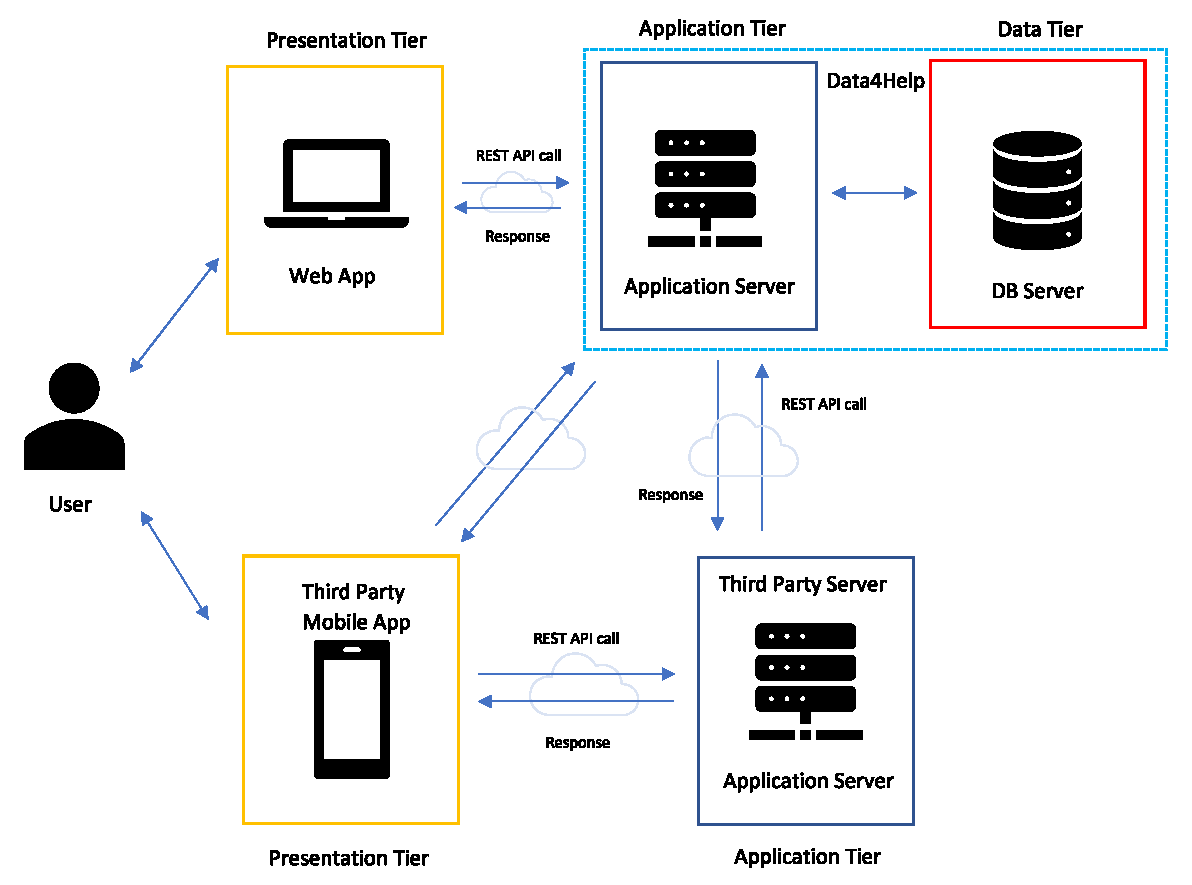
\includegraphics[width=\linewidth]{architecturalDesign-data4help}
    \caption{Data4Help system and its interaction with a generic third party}
    \label{fig:my_label}
\end{figure}

\begin{figure}[H]
    \centering
    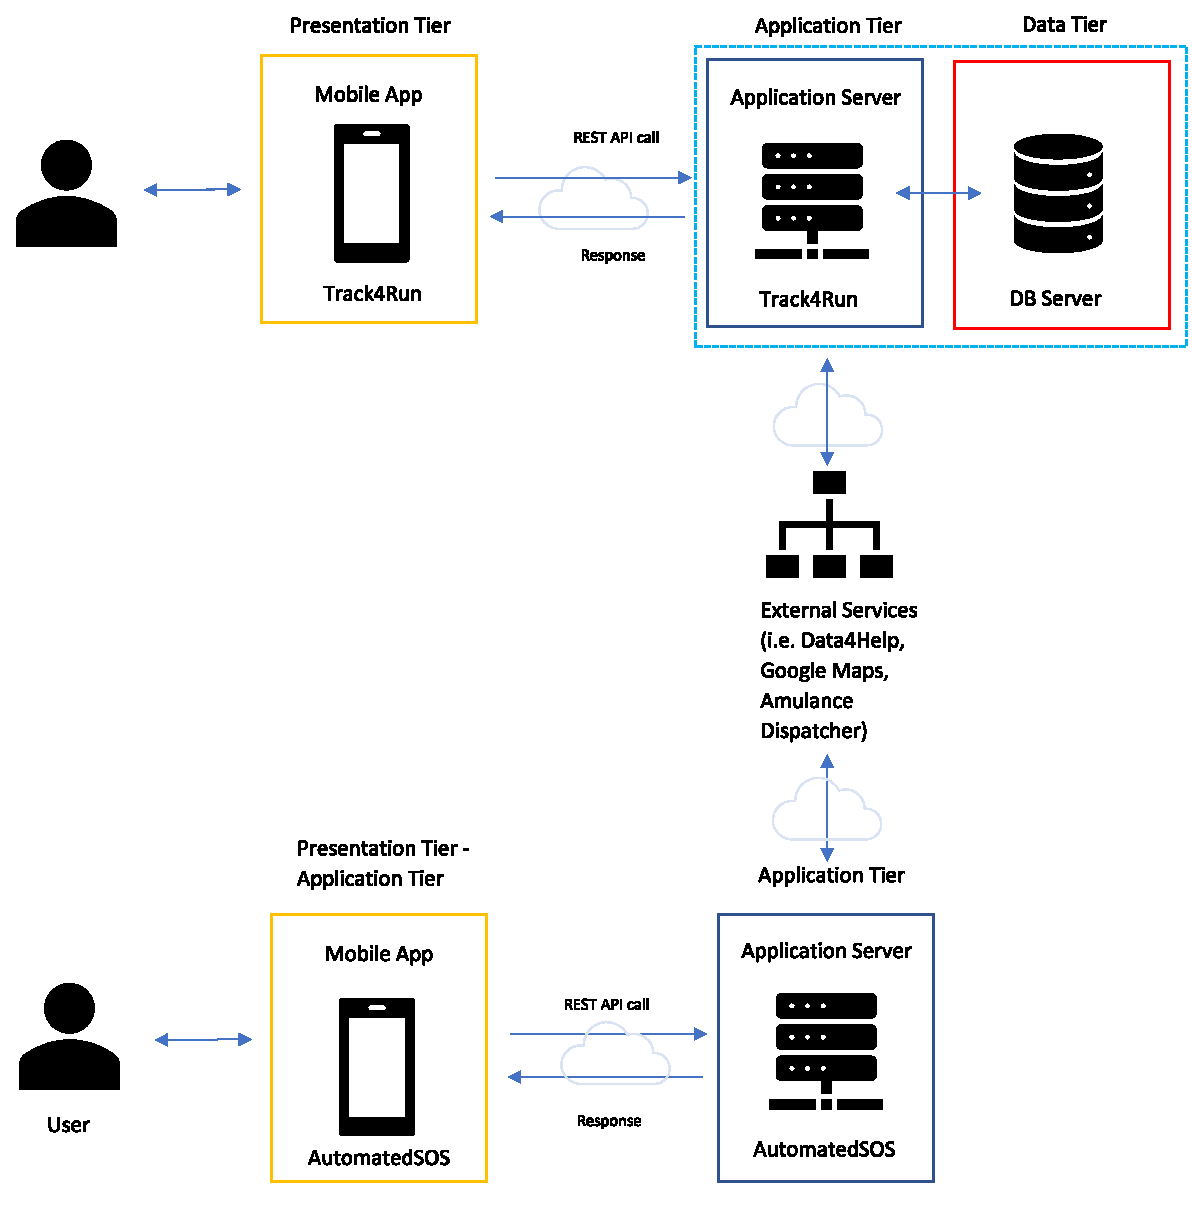
\includegraphics[width=\linewidth]{architecturalDesign-automated-track}
    \caption{AutomatedSOS and Track4Run structures communicating with external services.}
    \label{fig:my_label}
\end{figure}
The high-level components presented inside the diagrams are divided in different tiers in order to lighten the application on the user side and, at the same time, have a better control of the application logic and storage layers.\\
Precisely, the structure is composed by:\\ \\
\textbf{Presentation Tier:} this is the user interface layer which permits the interaction of customers with the service. It consists in a web application for Data4Help, that communicates with users through a web page and specific forms, and in a software for smartwear and smartphone for AutomatedSOS and Track4Run, which need a mobile interface available whenever the user wants.\\ \\
\textbf{Application Tier:} this is the application logic layer which contains the core of the software, composed by those functionalities and methods that are invoked from the user's interface to get the desired service.\\
In Data4Help system is the main part, because it performs the task of exchange data with third parties, handle individual and group permissions, save associations between users and third parties.\\
In AutomatedSOS, the application tier is split among client and server, because a specific function (the control of thresholds) is performed on the client-side, to get a lower response time. Instead, the data manager and the learning algorithm, which keeps in mind the differences between distinct users, is located on the server-side.\\
Finally, in Track4Run, it handles the different runs and allows to runners and spectators to join a specific event.\\ \\
\textbf{Data tier:} this is the storage layer, the one in which data are saved and are fetched from. It consists in a database which contains persistent elements and, for this reason, only Data4Help and Track4Run own it. Indeed, AutomatedSOS doesn't need a data tier because gets the data directly from Data4Help.
\clearpage

\subsection{Component View}
In this section the architecture is analyzed in a more detailed way, going deeper in the composition of the software structure and emphasizing the various typologies of service which make up the presentation and application logic layers.\\ \\
The main services of Data4Help are:
\begin{itemize}
    %Data4Help
    \item \textbf{RegistrationService:} handles the user's sign up, whether companies or individuals.
    \item \textbf{LoginService:} manages login and logout routines, available to users already registered.
    \item \textbf{RequestHandlerService:} sorts the requests depending on what they ask for, permissions or data (in this second case does already exists a permission that is a subscription or an individual one).
    \item \textbf{DataHandlerService:} interacts with the Data Collector API installed in third parties' applications and communicates with the database.
    \item \textbf{AnonymousPermissionMaker:} creates new anonymous permissions and handles requests for unsubscribe.
    \item \textbf{IndividualPermissionMaker:} creates new individual permissions and forwards requests to users which have to give the consensus.
    \item \textbf{AnonymousPermissionService:} handles subscription and sends requests of data to the interface communicating with the database.
    \item \textbf{IndividualPermissionService:}  handles individual permission and sends requests of data to the interface communicating with the database.
    \item \textbf{IndividualDataService:} communicates with the database to respond to individual data requests.
    \item \textbf{AnonymousDataService:} communicates with the database to respond to group data requests and controls if they can be anonymized.
\end{itemize}

\begin{sidewaysfigure}[h!]
    \centering
    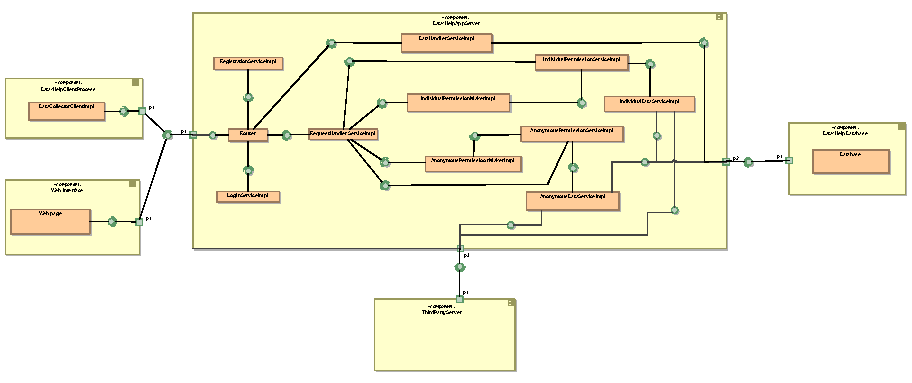
\includegraphics[width=\linewidth]{ComponentData4Help}
    \caption{Data4Help component view.}
    \label{fig:my_label}
\end{sidewaysfigure}
\clearpage

\noindent The most important services of AutomateSOS are:
\begin{itemize}    
    %AutomatedSOS
    \item \textbf{MonitorStatusService:} checks user's health status (on the client).
    \item \textbf{LearnThresholdsService:} gets user's data from Data4Help server and calculates specific user's thresholds.
    \item \textbf{EmergencyService:} notifies the ambulance dispatcher if the health status is below the thresholds.
\end{itemize}


\begin{figure}[H]
    \centering
    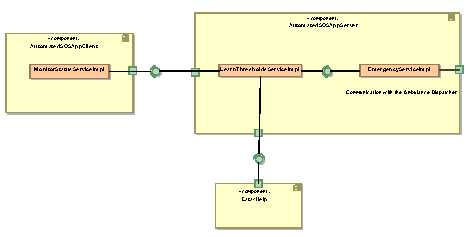
\includegraphics[width=\linewidth]{ComponentAutomatedSOS}
    \caption{AutomatedSOS component view.}
    \label{fig:my_label}
\end{figure}

\vspace{.5cm}
\noindent The principal services of Track4Run are:
\begin{itemize}    
    %Track4Run
    \item \textbf{RunCreationService:} allows organizers to create a run event.
    \item \textbf{RunManagementService:} manages a specific run event, adding and removing participants and editing the path.
    \item \textbf{RunTrackingService:} obtains runners' positions during a run event.
    \item \textbf{RunWatchService:} handles the spectators and updates views during a run event.
\end{itemize}

\begin{figure}[H]
    \centering
    \includegraphics[width=\linewidth]{Component-Track4Run}
    \caption{Track4Run component view.}
    \label{fig:my_label}
\end{figure}

\vspace{.5cm}
\noindent The previous schemata represent the implementation of the interfaces containing those methods which allow to access to listed services. \\ 
The \textit{Router} has the duty to sort requests and messages which arrive to the server port. It is a generic interface and it doesn't assume a specific aspect because it could work like a middleware or be a simply interfaces built on top a socket communication. This decision is purely an implementation detail.\\ \\ \\
The following two diagrams illustrate the relationships inside the application logic of the entire system, considering also AutomatedSOS and Track4Run services, and give a more precise idea of the involved classes and interfaces from which are used.\\
The first diagram is simply a class diagram, generated from the one illustrated in the RASD and enriched with more precise classes and concepts, useful to split some specific components and favor cohesion inside the system.\\
Instead, the second diagram is an anticipation of the section 2.6, in which are explained the component interfaces. Indeed, the schema shows the \textit{use} relationships between the service interfaces and the main classes of the system. It also permits to have a clearer hint about the complete system and it can be useful to better understand the runtime views.  

\begin{sidewaysfigure}
    \centering
    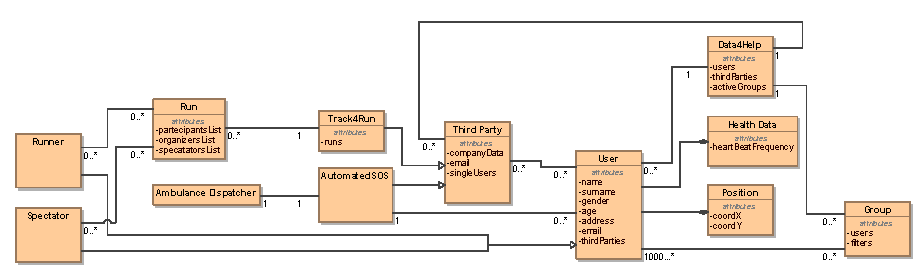
\includegraphics[width=\linewidth]{classDiagram}
    \caption{UML Class Diagram of the whole system.}
    \label{fig:my_label}
\end{sidewaysfigure}

\begin{figure}[H]
    \centering
    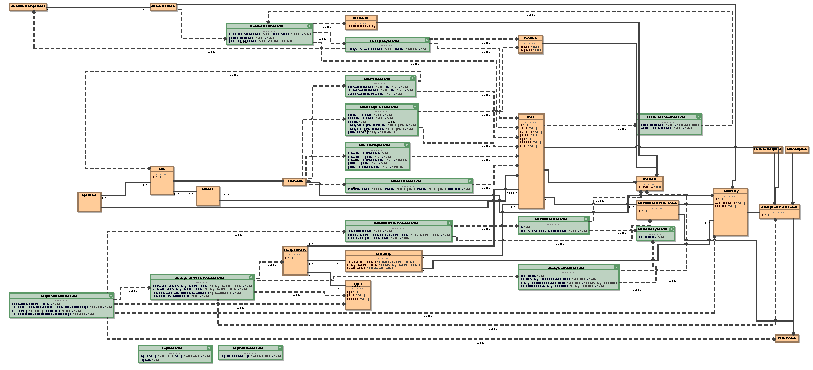
\includegraphics[width=\linewidth, height=\textheight]{ClassDiagramTotal}
    \caption{UML Class Diagram of the whole system.}
    \label{fig:my_label}
\end{figure}
\clearpage

\subsection{Deployment View}
The Deployment diagram focuses on how the software is deployed to the target nodes. For convenience this section is split in three parts, one for each software product.

\paragraph{Data4Help}
This section is devoted to Data4Help analysis. \\
First of all, the Data4Help Data Collector Process, which is the software component that collects data from smart devices, is installed on the user's smartphone. \\
In this node there is a relation of composition with a generic Third Party application, that exploits the service provided by Data4Help using the API for data collection. \\
The artifact, actually, is not available in a stand alone version, but it has to be included in the app that will use the Data4Help service. \\
We made this choice because we think that the service offered by Data4Help is useful only when a third party application (such as AutomatedSOS and Track4Run do) requires user's data, otherwise is not reasonable to think that a user will install only the Application for sharing his/her own data. \\
Another aspect that needs to be clarified is that the Sensor Data Collector artifact is an ad-hoc software developed by the smart device manufacturer and not by TrackMe, so it has been added for better understand the environment in which the process on the client-side will operate. \\
It is also available a web interface for Data4Help in order to manage credentials and, for what concerns the third parties, ask for user's data. \\
The server side of the application contains the business logic, such as the permissions management and the data anonymizing process, and it is deployed on the Data4Help Server component which also interacts with a dedicated database.

\begin{figure}[H]
    \centering
    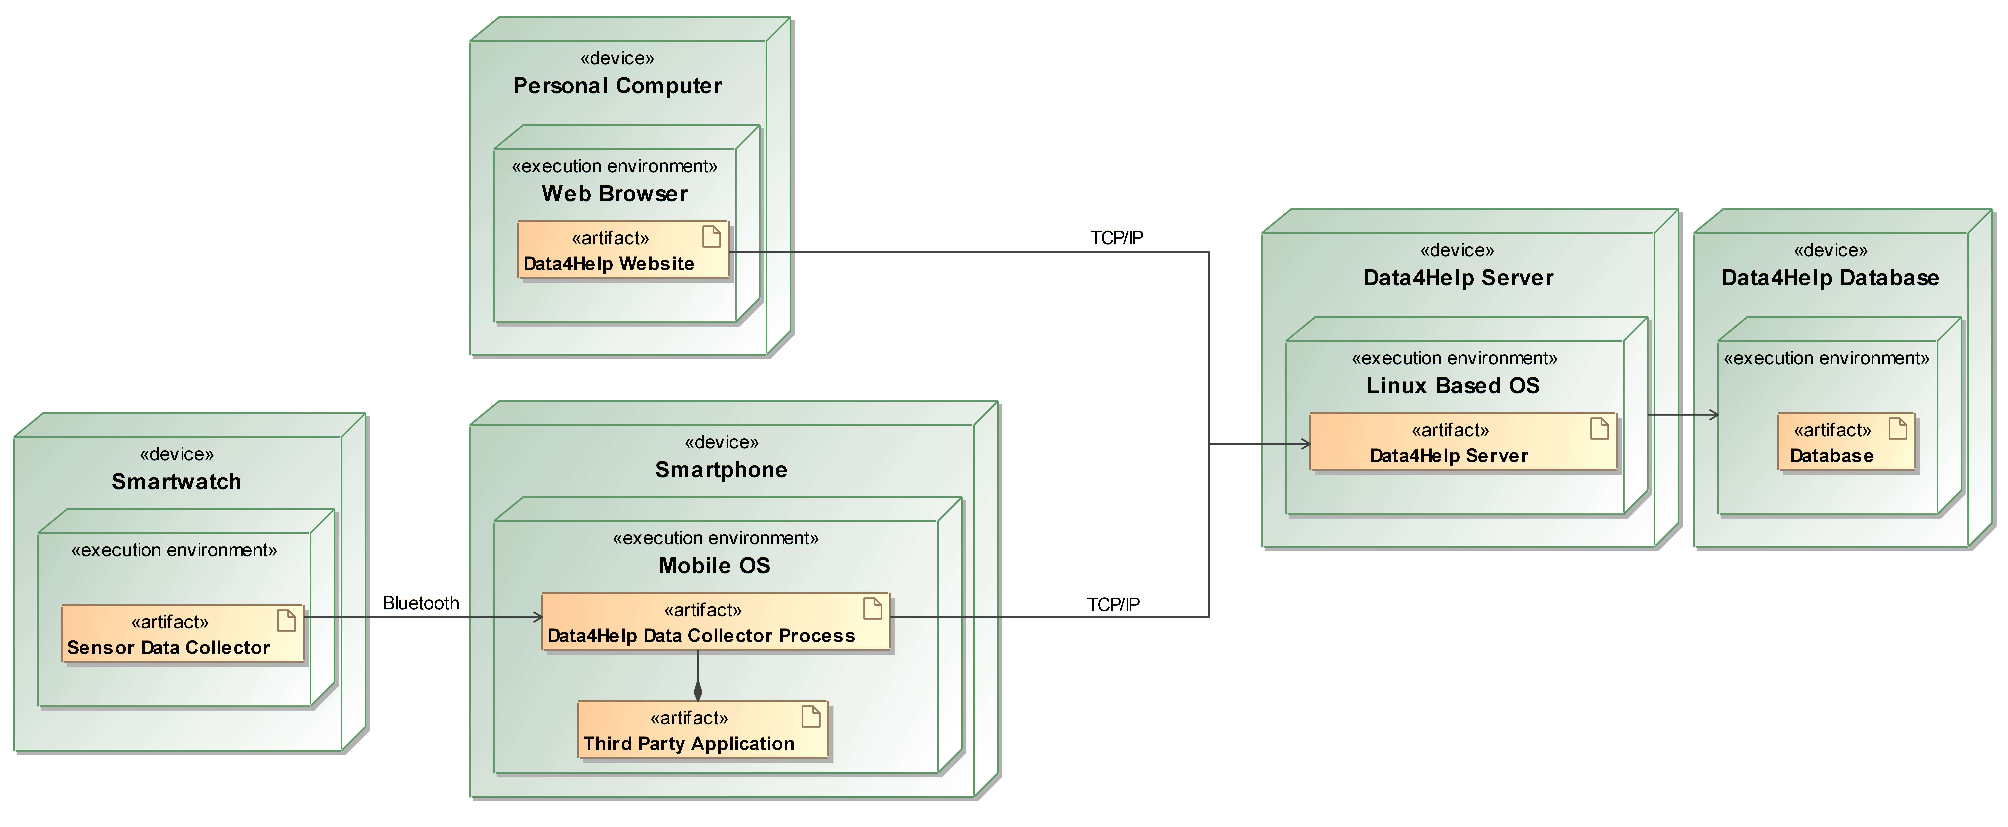
\includegraphics[width=\linewidth]{deploymentDiagram-Data4Help}
    \caption{Deployment Diagram of Data4Help system.}
    \label{fig:my_label}
\end{figure}

\paragraph{AutomatedSOS}
AutomatedSOS is designed as a third party application in order to reuse the same software stack built over Data4Help. \\
Since AutomatedSOS is built on top of Data4Help, is necessary to deploy the Data Collector Process in the user's smartphone. \\
The user can also install an additional app on his/her smartwatch to see the health status in real time. The artifact deployed on the smartphone calculates in background if the health parameters are acceptable with respect to the threshold values.\\
On the server-side the AutomatedSOS server handles the emergency message sent by the smartphone and it notifies the Ambulance Dispatcher. \\
Another functionality implemented on the server is the computation of the threshold values for each distinct user which will be sent to the smartphone application.

\begin{figure}[H]
    \centering
    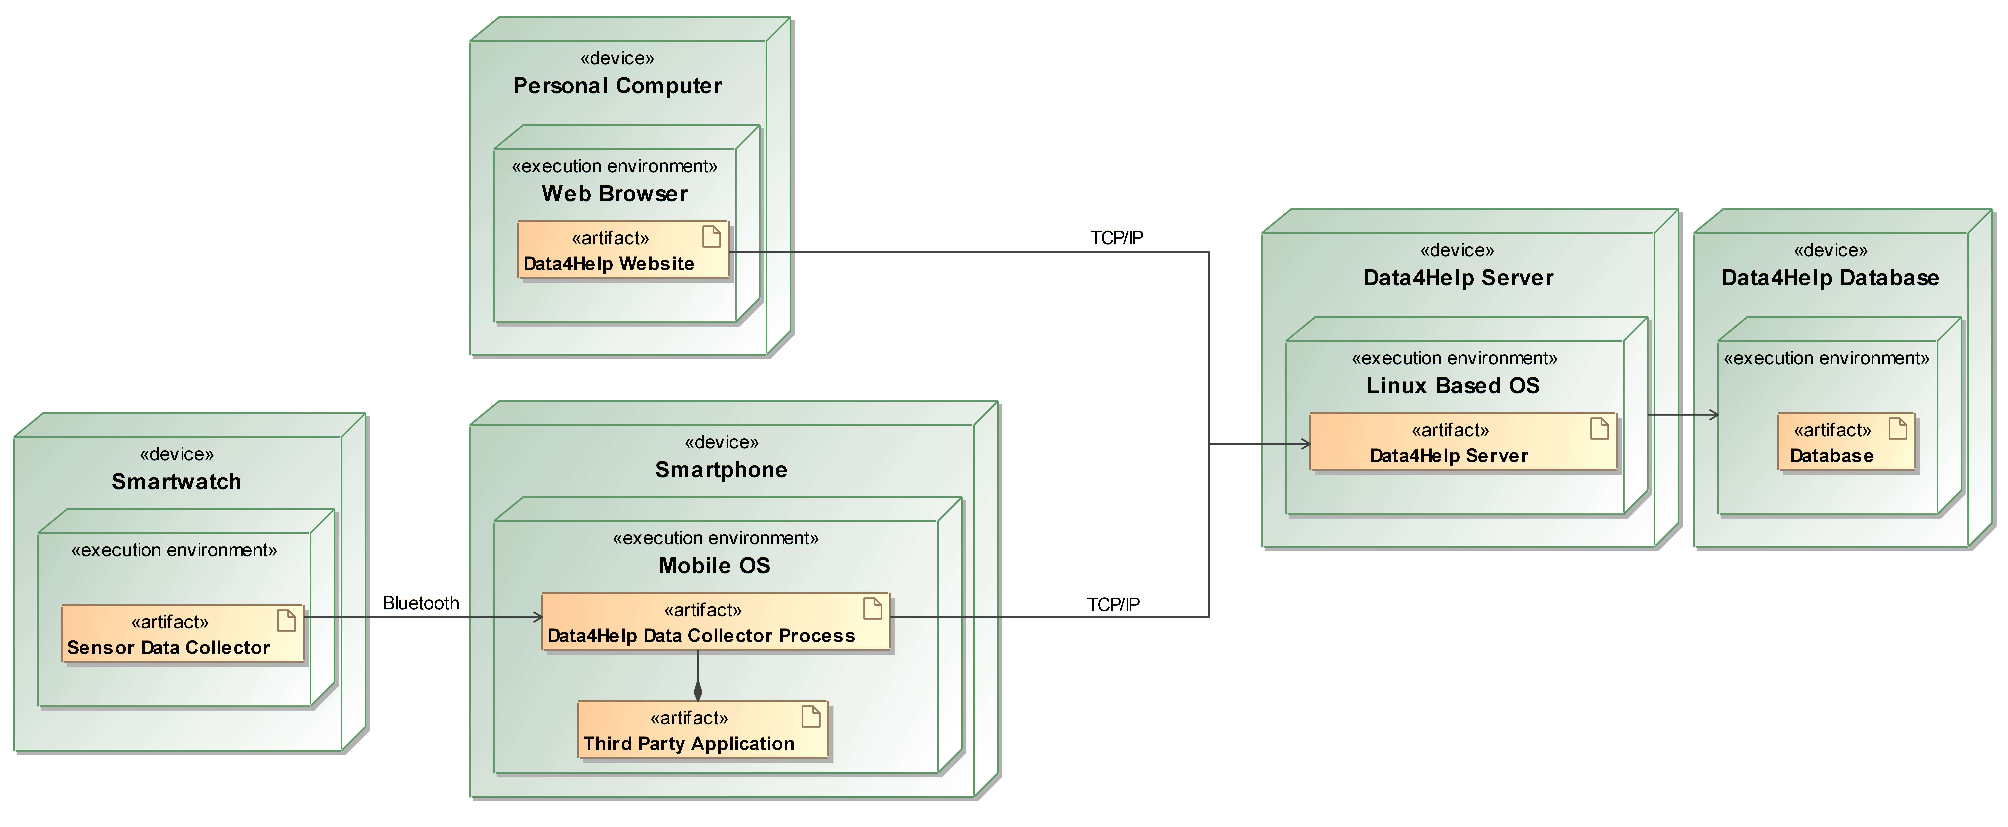
\includegraphics[width=\linewidth]{deploymentDiagram-AutomatedSOS}
    \caption{Deployment Diagram of AutomatedSOS system.}
    \label{fig:my_label}
\end{figure}

\paragraph{Track4Run}
Track4Run is built on top of Data4Help as AutomatedSOS, so previous considerations are valid also for this application. The smartphone app allows the user to create, enroll and watch a run by communicating with the Track4Run server. \\
It is also responsible for retrieving data from the external map service (in this case Google Maps) and to mirror the major information, like the path during a run on the smartwatch app. \\
The server app handles the management of the run, the request of the spectator, giving them the updated runner's position, and all the routines which precede the start of the run event.

\begin{figure}[H]
    \centering
    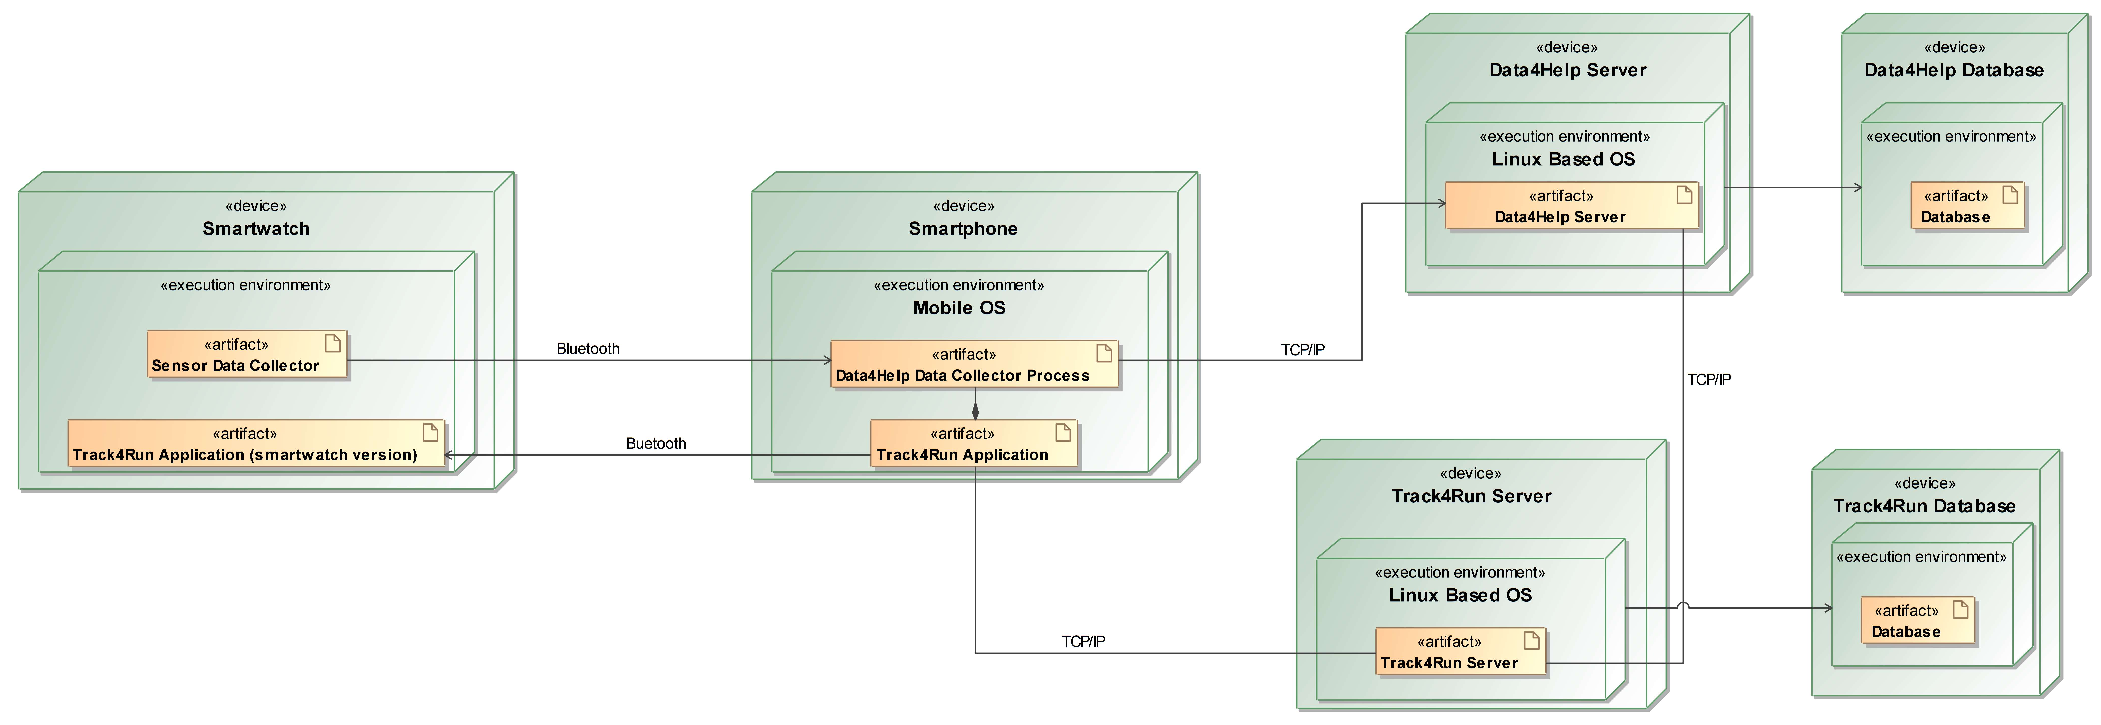
\includegraphics[width=\linewidth]{deploymentDiagram-Track4Run}
    \caption{Deployment Diagram of Track4Run system.}
    \label{fig:my_label}
\end{figure}
\clearpage

\subsection{Runtime View}
Before the beginning of the runtime analysis, there is a note that has to be clarified: not all the message types that appear in the sequence diagrams are represented in the class diagram because they are used as wrappers for different data type (i.e. retrieving a user tuple from the database).

\subsubsection{Data4Help - Third Party requires the permission to access to individual user data}
This sequence diagram shows the case in which a third party requires the access to specific user's data and how the system manage the permission. \\
The third party, through the web interface or through its app, requires for the permission, indicating the users involved.\\
A permission request is sent to the Data4Help Server, where the RequestHandlerService manages it and invokes the creation of the individual permission in the IndividualPermissionMaker. This service shall forward the request, that has to be accepted or refused from the user, and receives the response. If the user allows to share his data, the permission is stored in the IndividualPermissionService and finally the Third Party is notified that the request is accepted.\\
On the contrary, if the user refuses to share his data it is not stored any permission in the system and the third party is notified that the request is not accepted.

\begin{figure}[H]
    \centering
    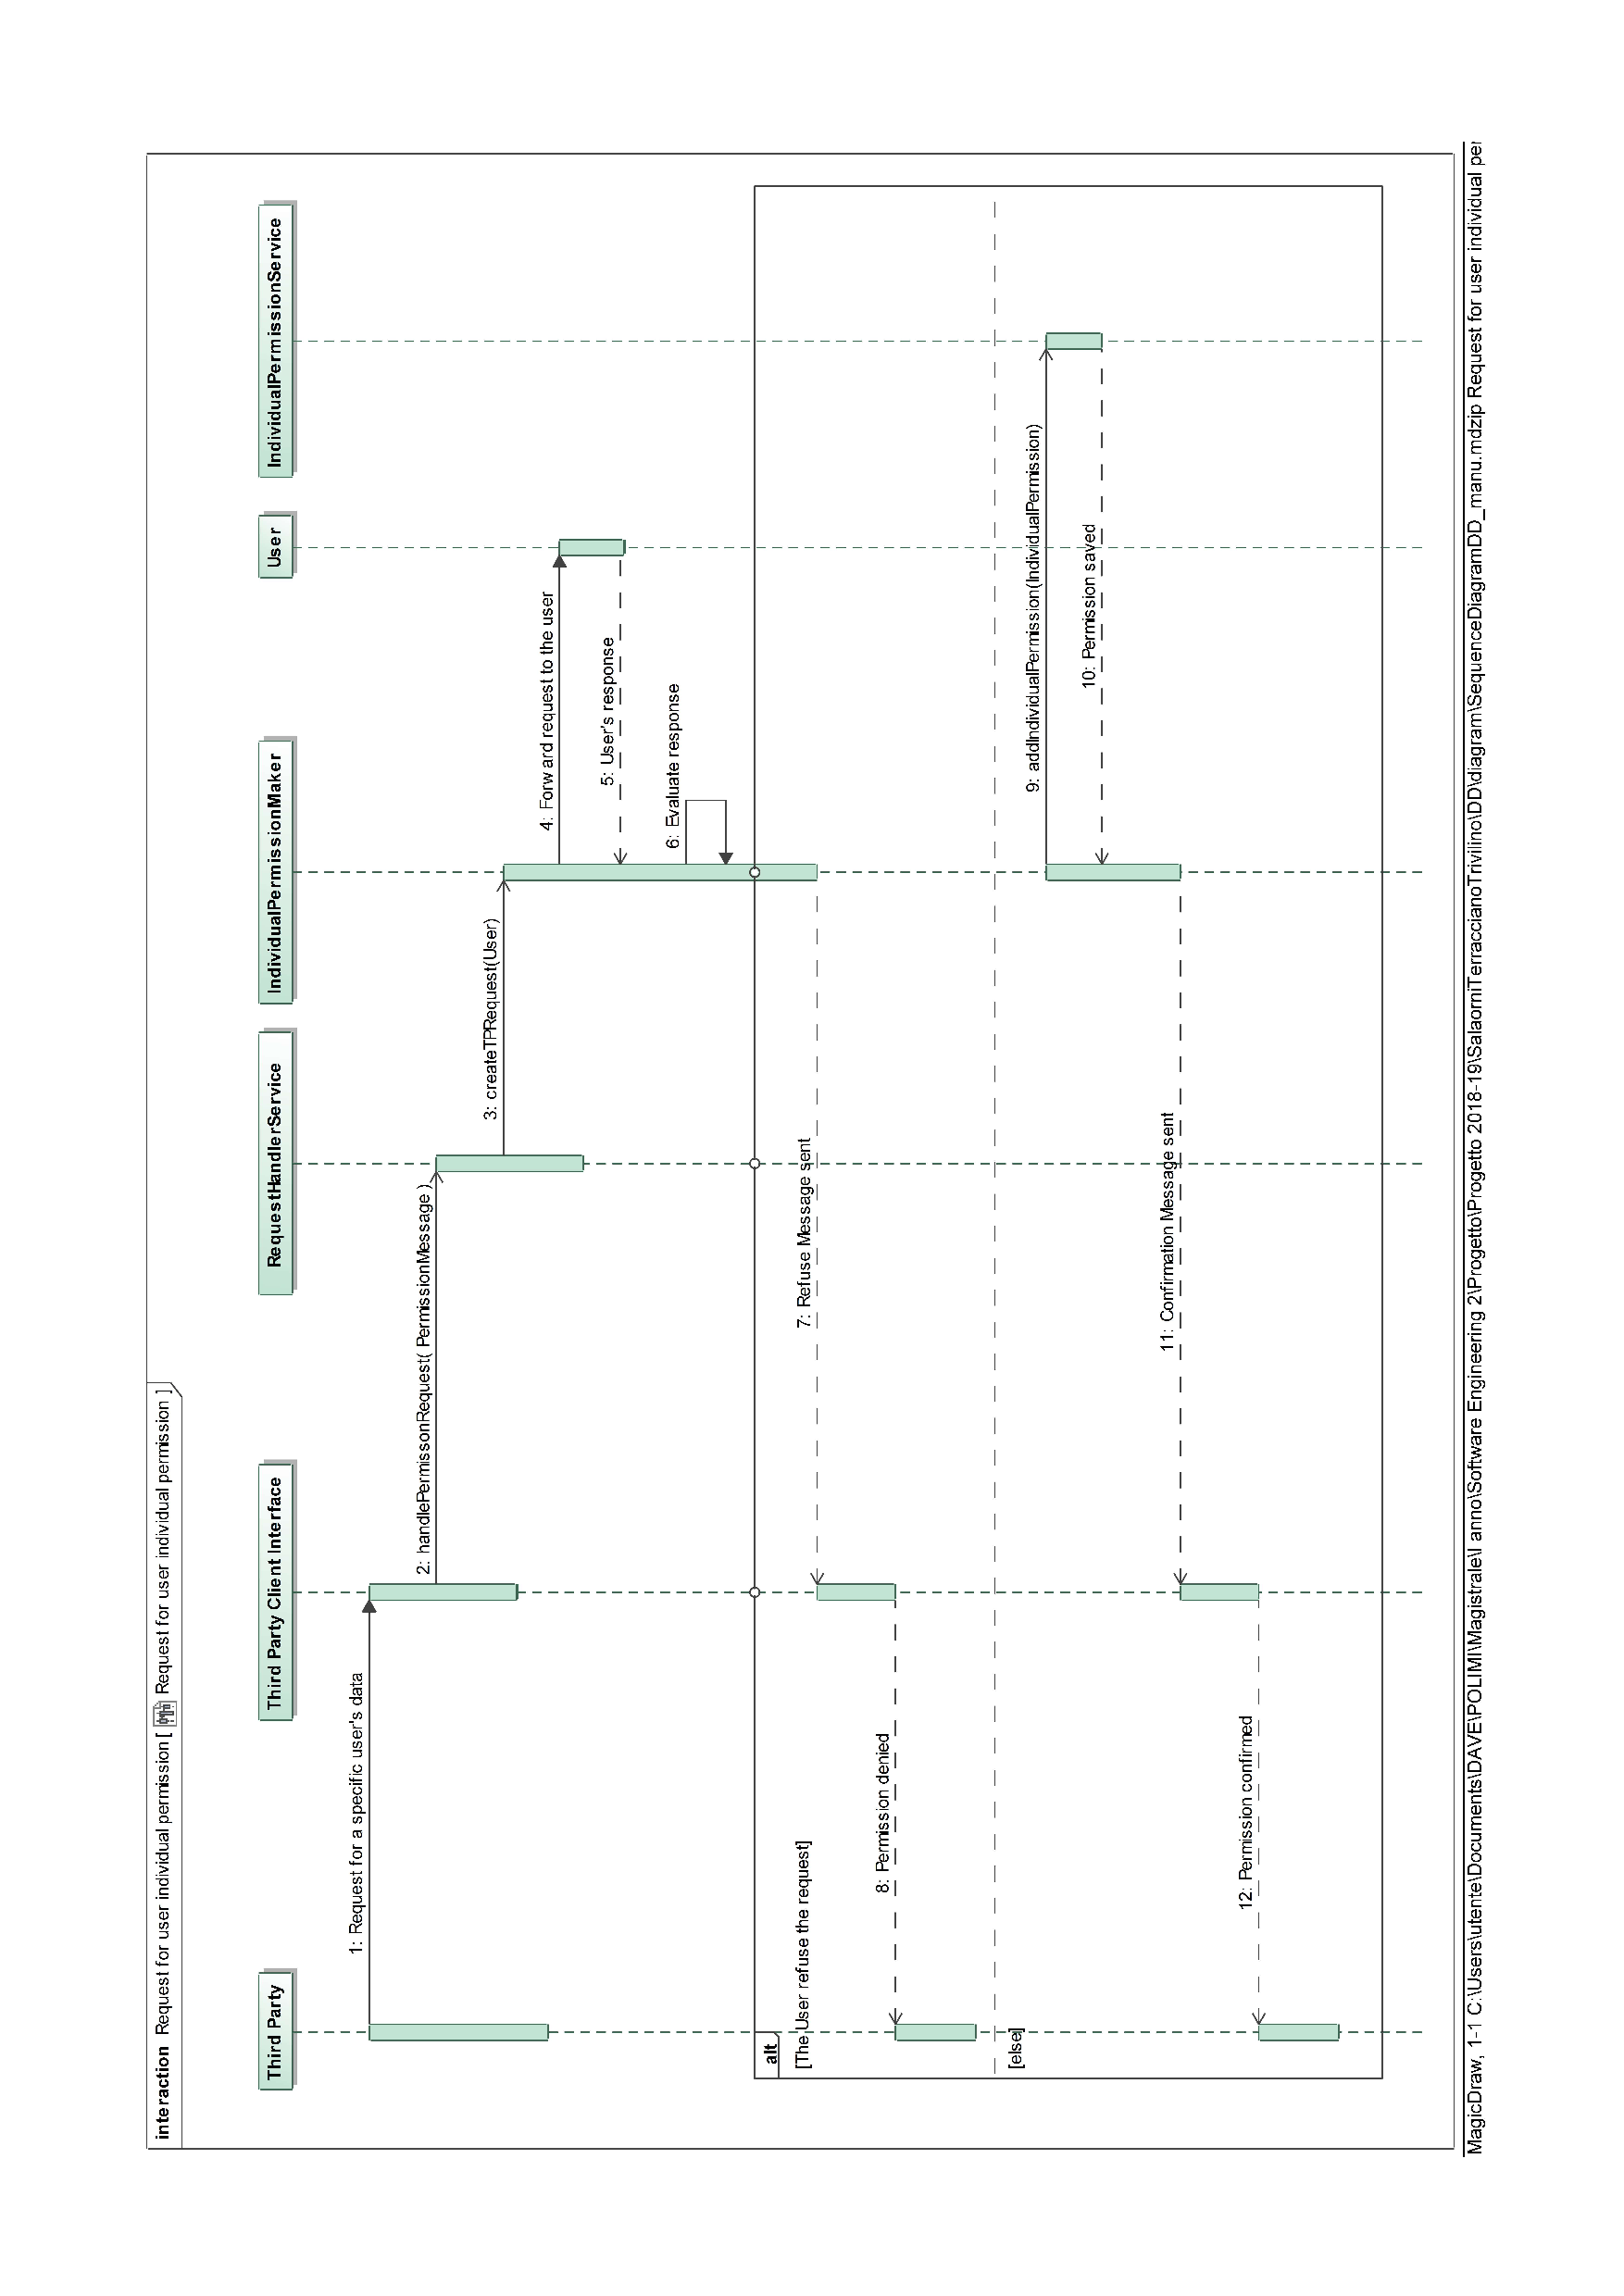
\includegraphics[width=\linewidth]{SequenceDiagram-RequestForUserIndividualPermission}
    \caption{Sequence Diagram showing the runtime flow.}
    \label{fig:my_label}
\end{figure}
\clearpage

\subsubsection{Data4Help - Third Party acquire individual user data}
This sequence diagram shows the case in which a third party requires to some individual user's data. \\
The third party, through the web interface or through its app, requires for the data, indicating the user. \\
A data request is sent to the Data4Help Server, where the RequestHandlerService manage it and check in the IndividualPermissionService if the related permission already exists. \\
If the permission does not exist the process to create a new permission is invoked (see previous sequence diagram). Otherwise if the permission already exists, the RequestHandlerService invokes the IndividualPermissionService to fetch and send the data and finally the IndividualDataService sends to the Third Party the required data.

\begin{figure}[H]
    \centering
    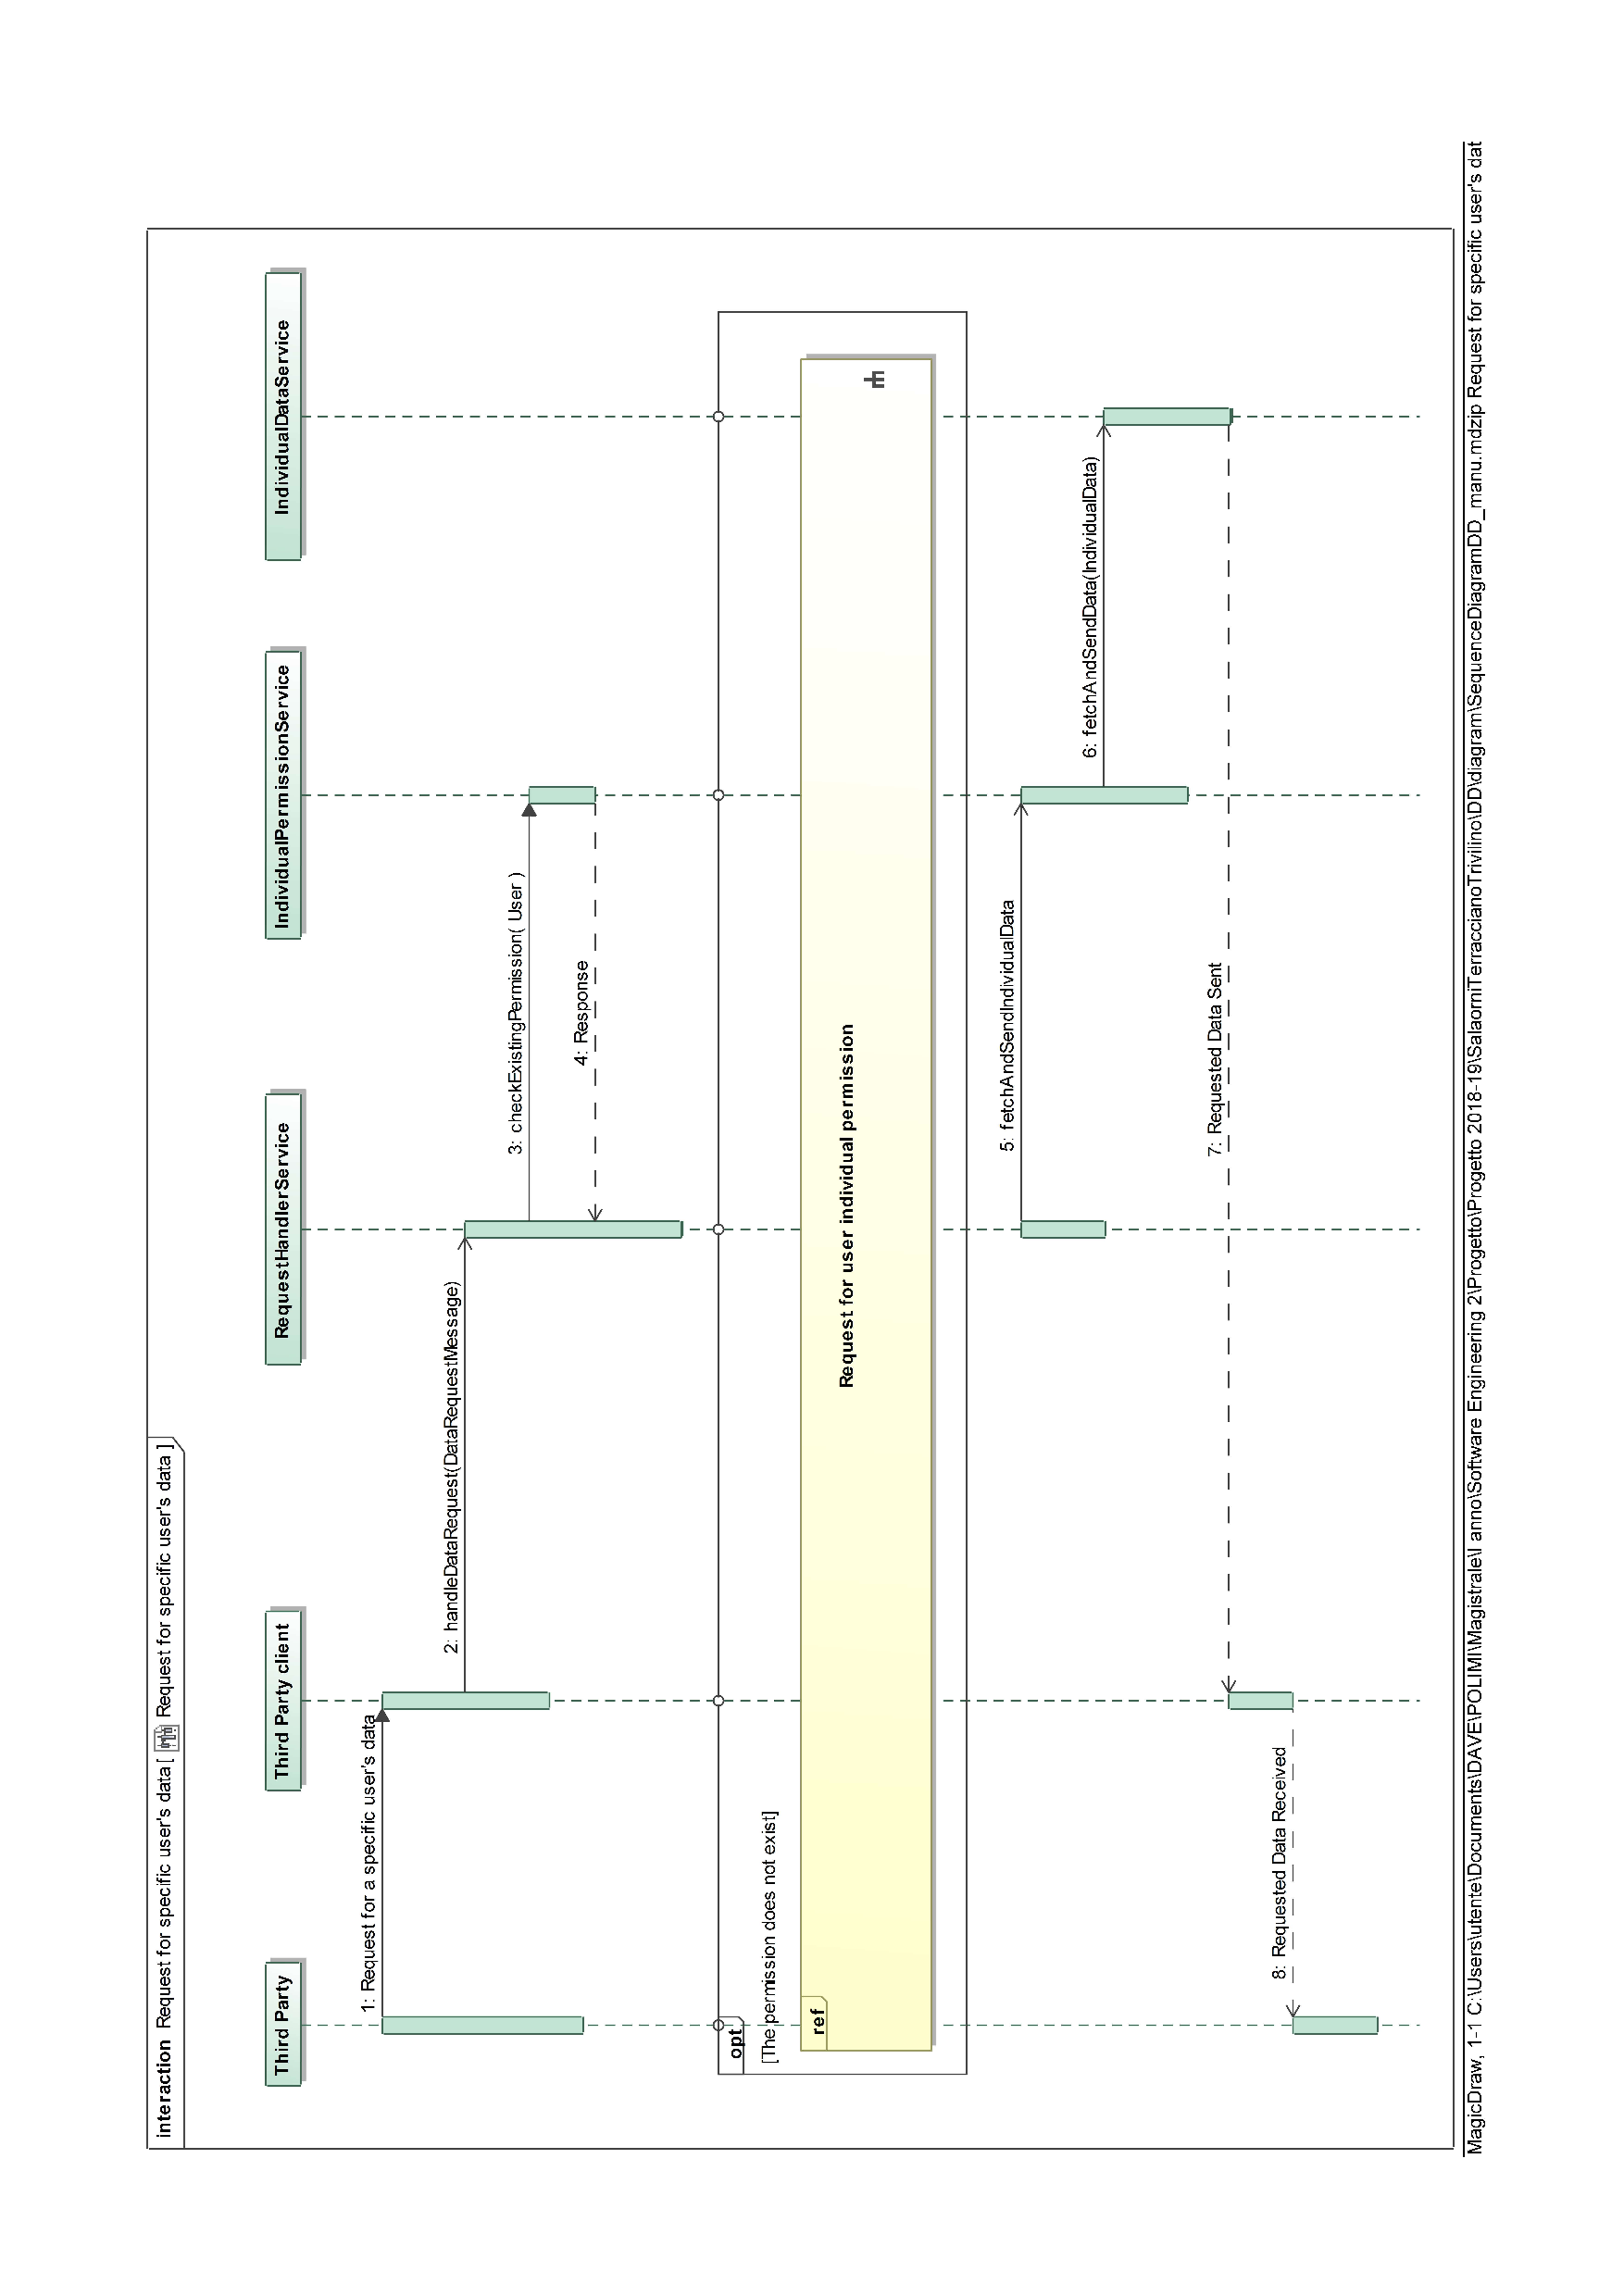
\includegraphics[width=\linewidth]{SequenceDiagram-RequestForSpecificUserData}
    \caption{Sequence Diagram showing the runtime flow.}
    \label{fig:my_label}
\end{figure}
\clearpage

\subsubsection{Data4Help - Third Party requires anonymized group data}
This sequence diagram shows the case in which a third party requires to some anonymized data from a group of target users. \\
The third party, through the web interface or through its app, requires for the data, indicating the filters and the target to group the users. \\
A permission Request is sent to the Data4Help Server, where the RequestHandlerService manage it and invoke the creation of the anonymous permission in the AnonymousPermissionMaker. \\
The AnonymousPermissionMaker then requires the data for the "one-shot" request to the AnonymousDataService that check if the data can be anonymized or not, if it is possible the data is sent to to the third party. Otherwise the third party is notified that it is not possible to share data and guarantee the user anonymity.

\begin{figure}[H]
    \centering
    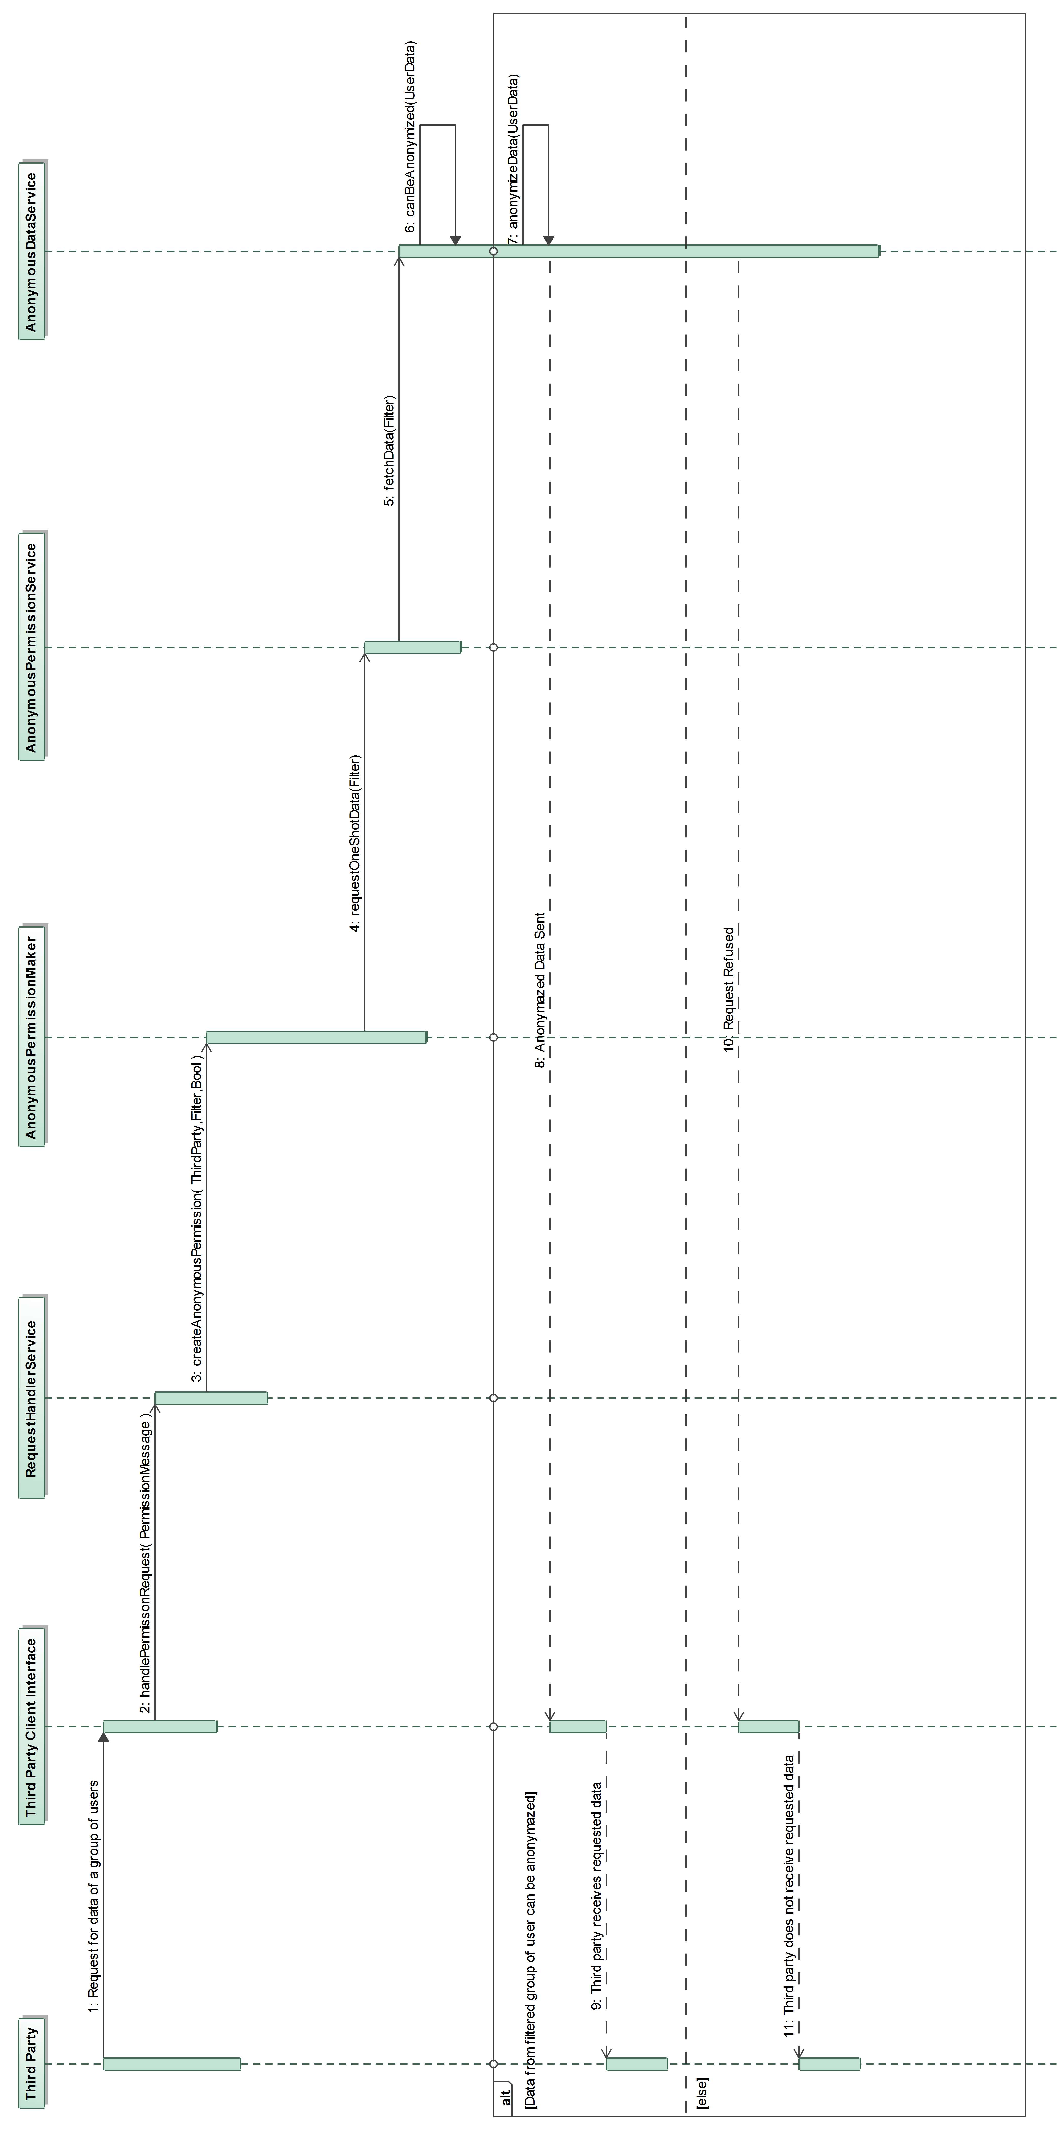
\includegraphics[width=\linewidth, height=\textheight]{SequenceDiagram-RequestForAnonymizedData}
    \caption{Sequence Diagram showing the runtime flow.}
    \label{fig:my_label}
\end{figure}
\clearpage

\subsubsection{Data4Help - Third party subscribes to anonymized data}
This sequence diagram shows the case in which a third party requires some anonymized data from a group of target users. \\
The third party, through the web interface or through its app, requires for the data, indicating the filters and the target to group the users. \\
A permission request is sent to the Data4Help Server, where the RequestHandlerService manages it and invokes the creation of the anonymous permission in the AnonymousPermissionMaker. \\
Then, the AnonymousPermissionMaker invokes the AnonymousPermissionService to store the subscription permission.\\
Data are sent to the third party, as already described in the anonymous data request, periodically, until the third party unsubscribes. 

\begin{figure}[H]
    \centering
    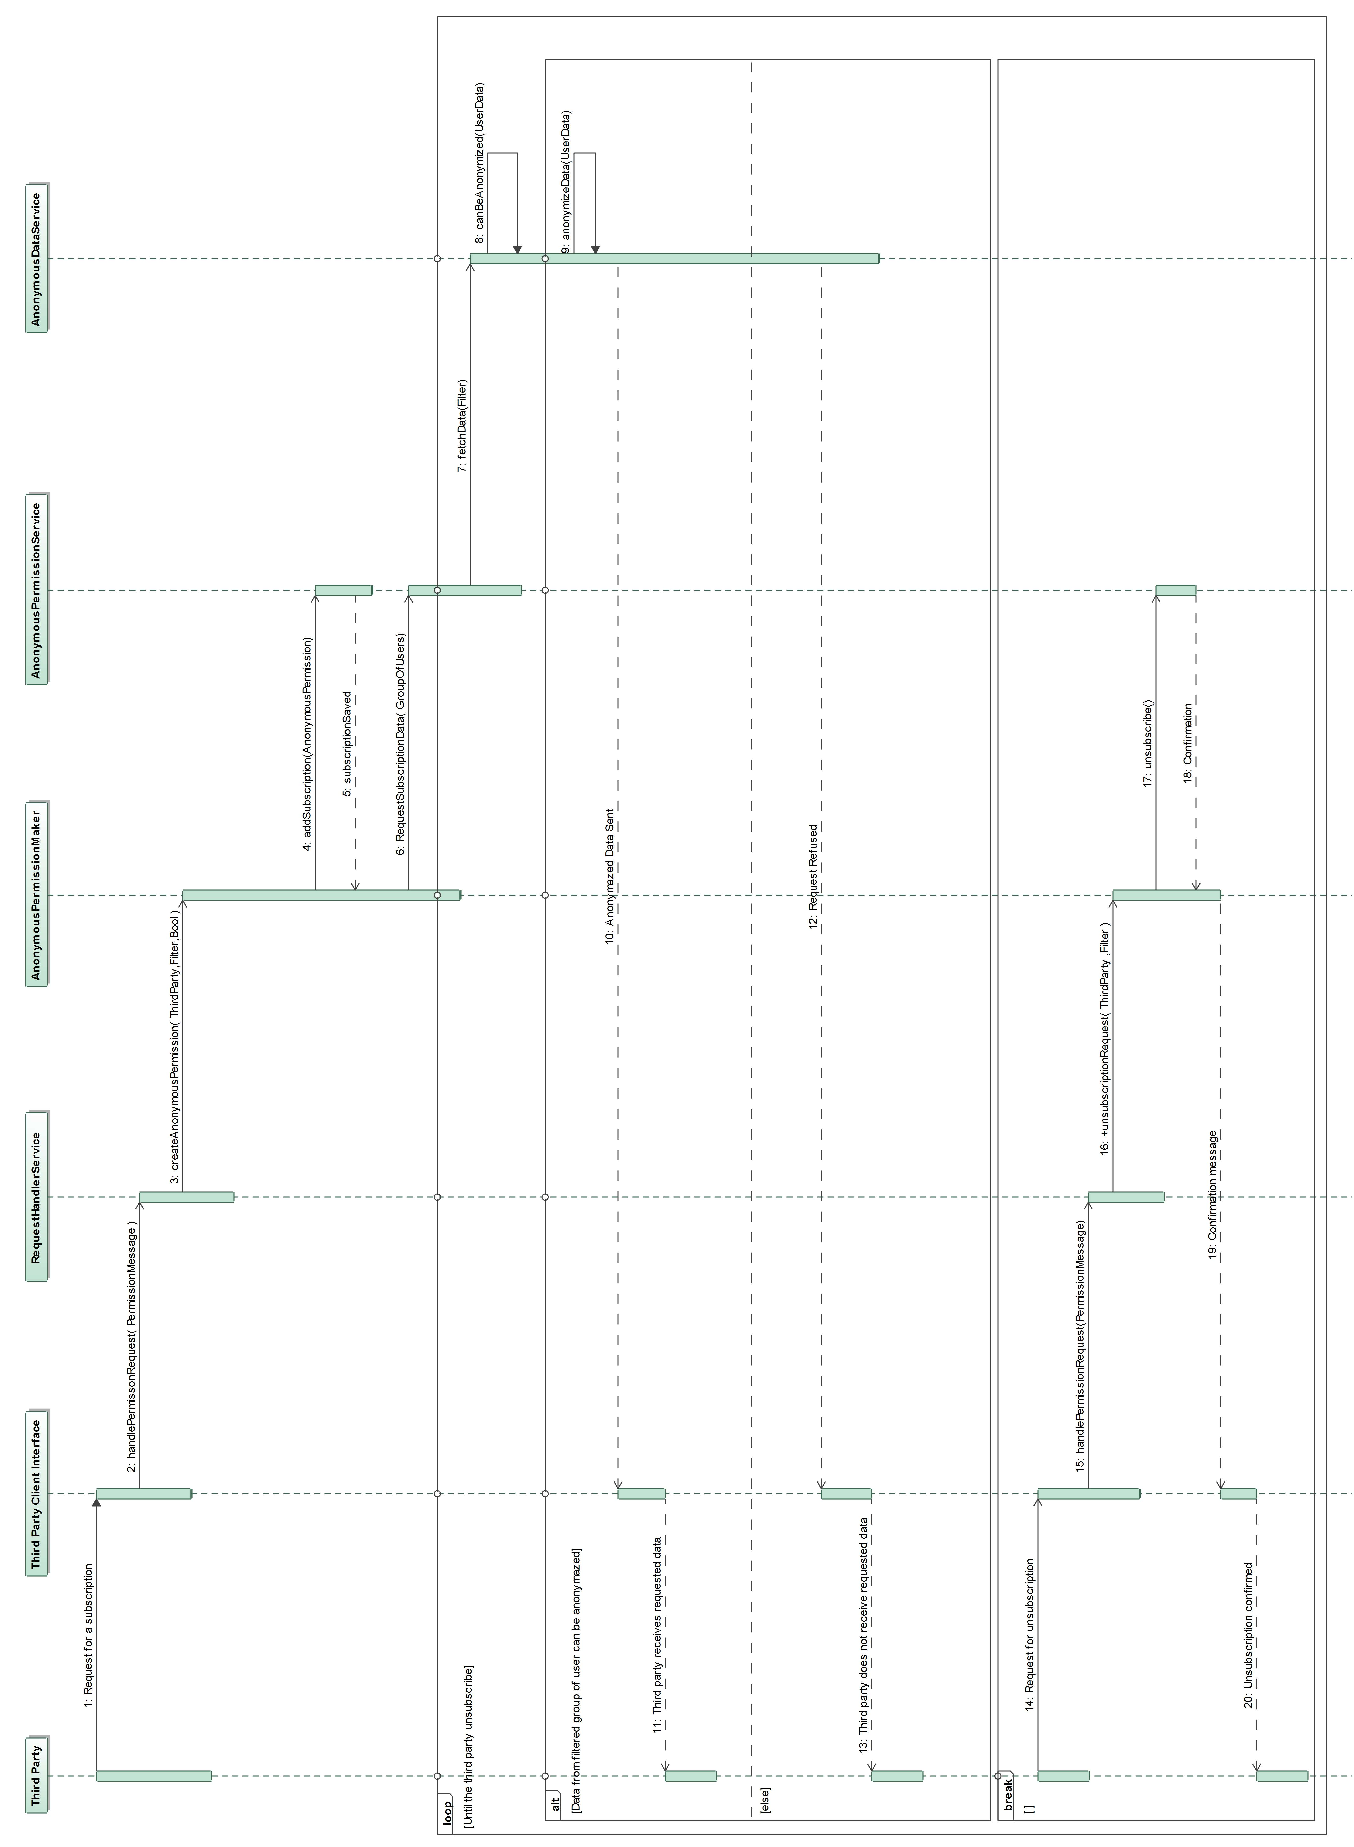
\includegraphics[width=\linewidth]{SequenceDiagram-RequestForSubscription}
    \caption{Sequence Diagram showing the runtime flow.}
    \label{fig:my_label}
\end{figure}
\clearpage

\subsubsection{AutomatedSOS - Alert Emergency Status}
The diagram shows the routine executed by AutomatedSOS when a user enters in the emergency status. \\
After the request of the user health status to the Data4Help Data Collector Process the application compares them with their threshold values and, once it has verified that the safety constraint is not respected, contacts the Emergency Service sending the User and his/her current position. \\
A notification is sent periodically until the receipt of the ack from the Emergency Service and, after that, the user is informed that an ambulance has been called.\\
Otherwise, if the user is not in danger, the health status is regularly showed in the application.

\begin{figure}[H]
    \centering
    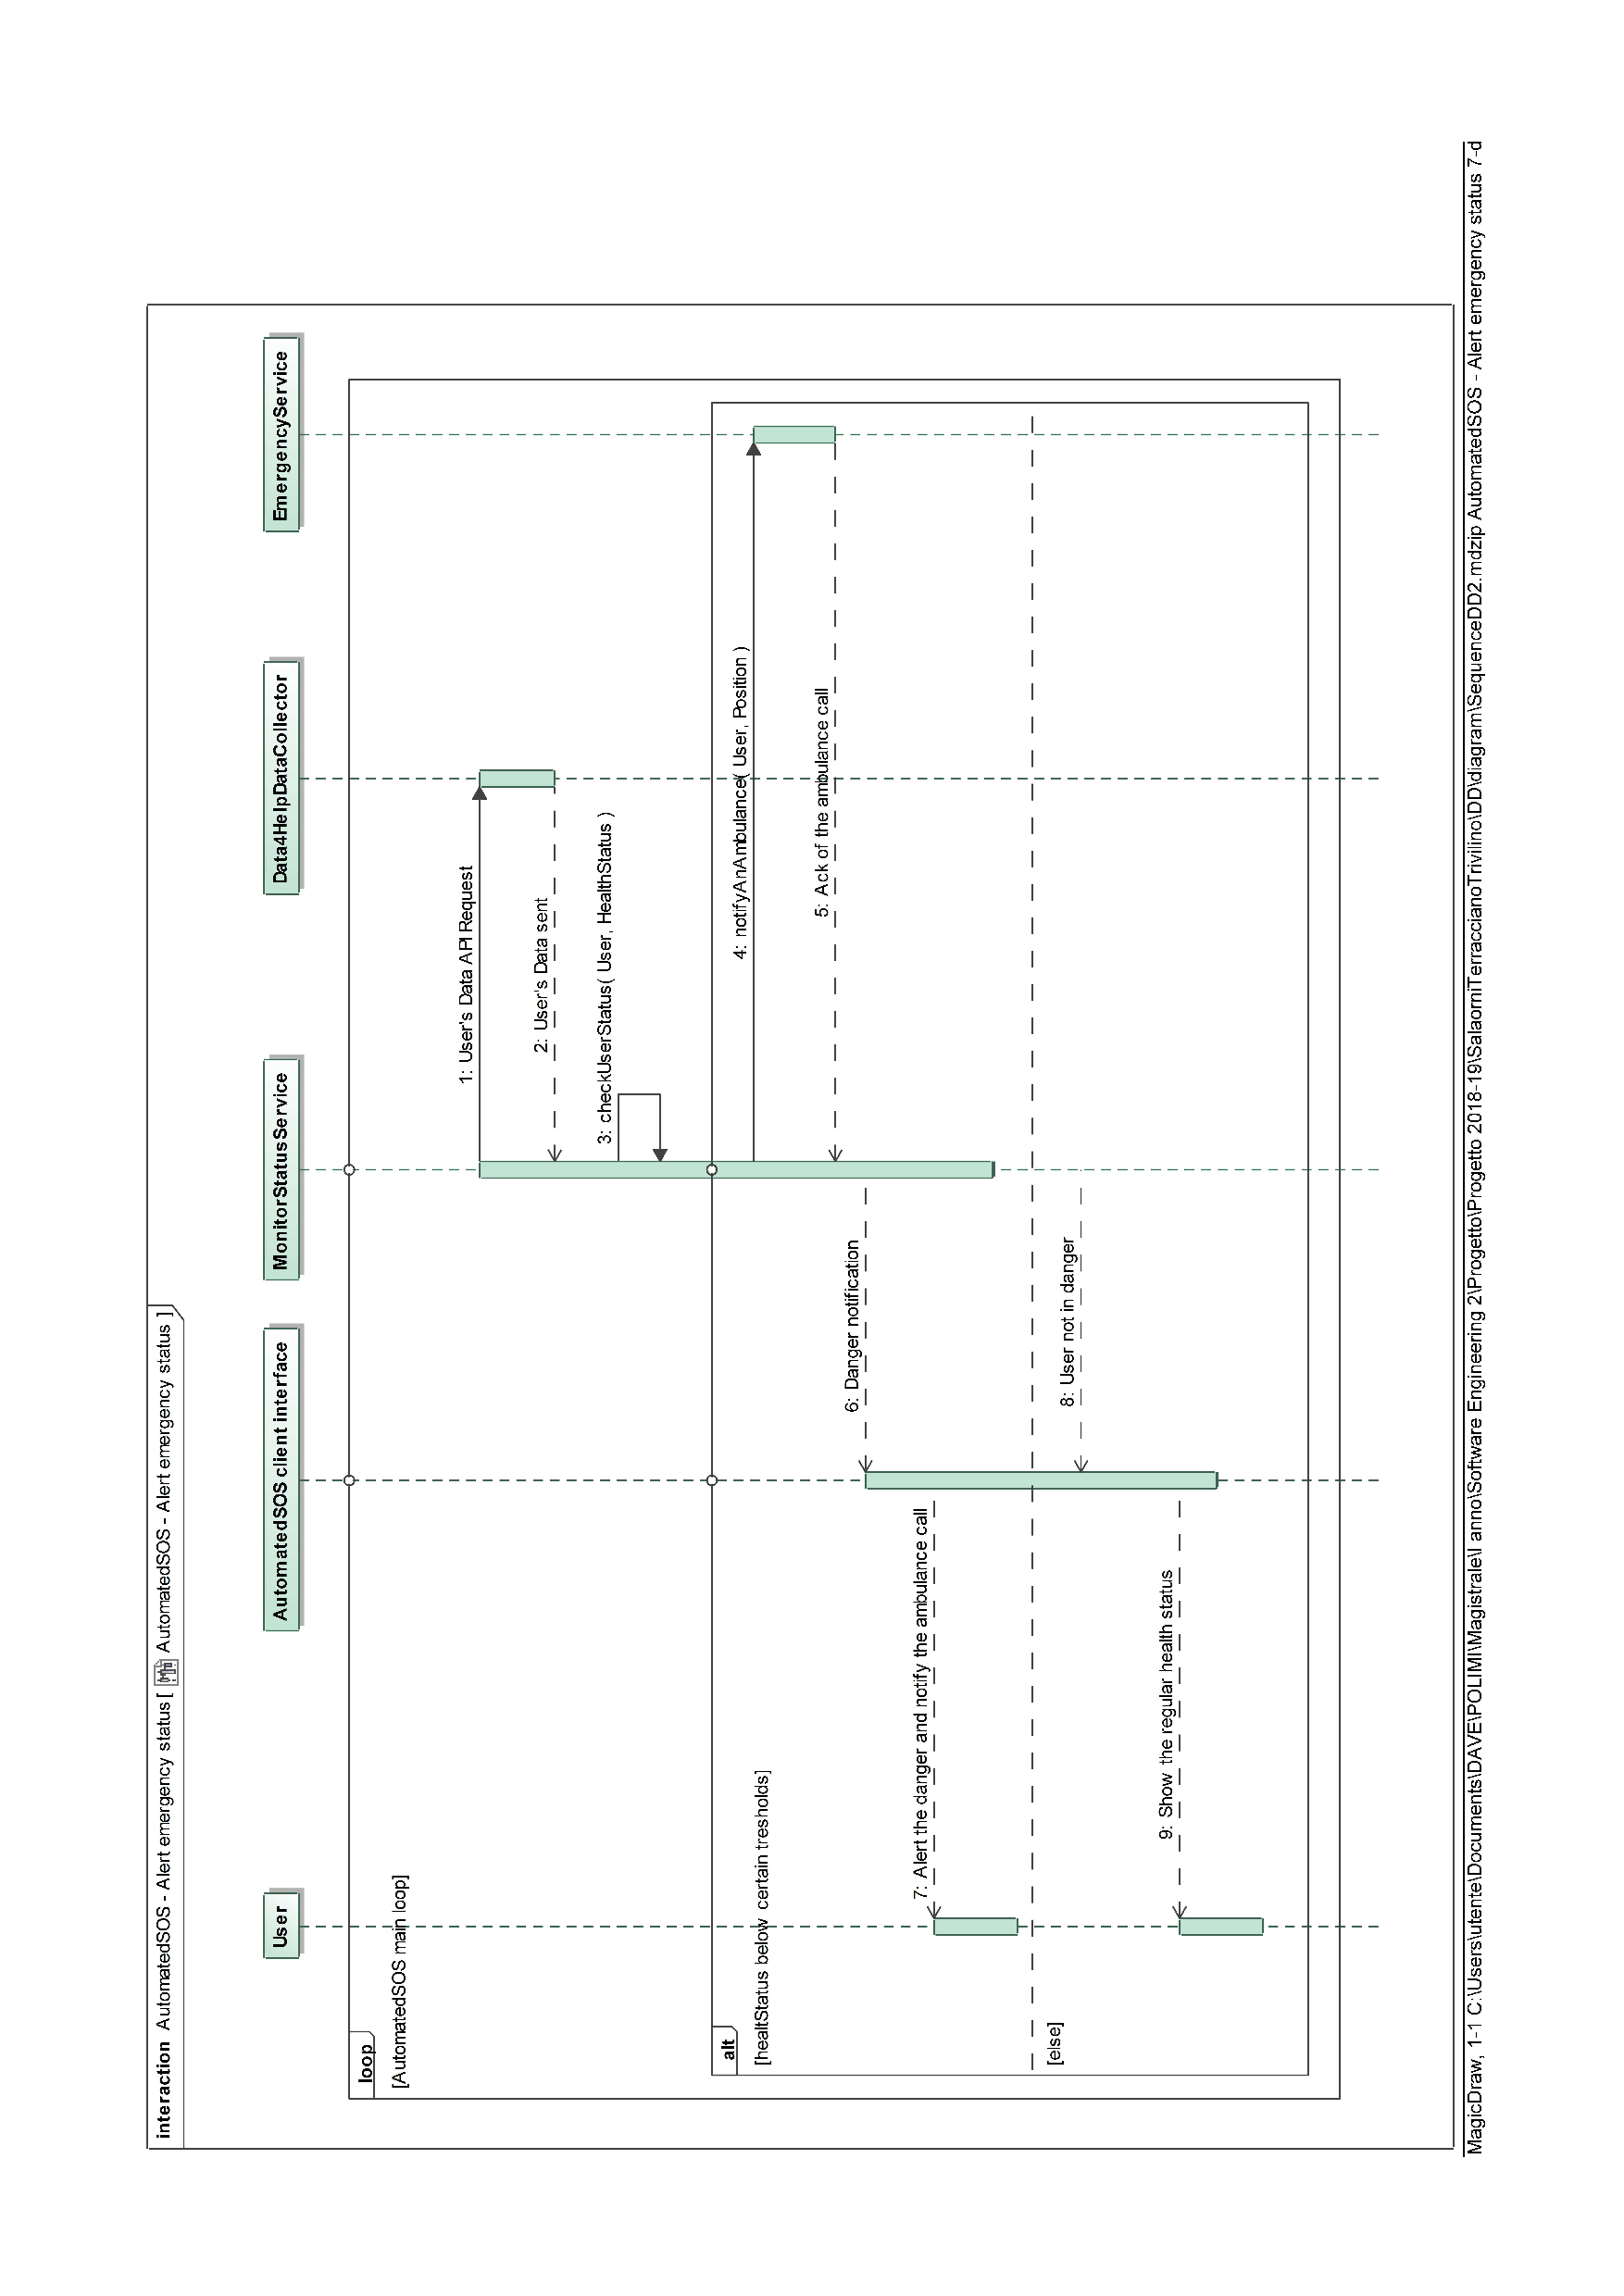
\includegraphics[width=\linewidth]{SequenceDiagram-AlertEmergencyStatus}
    \caption{Sequence Diagram showing the runtime flow.}
    \label{fig:my_label}
\end{figure}
\clearpage

\subsubsection{Track4Run - Create and enroll in a run}
The creation of a run start with a specific request sent from the mobile application in which are specified the user, the starting and ending point, the date and the hour at which the run will start. \\
Concerning the enrollment, the user will search from the mobile application through the list of available runs the one in which he/she wants to enroll. \\
Thus, the user is added to the runner of the event and will receive a confirmation message.

\begin{figure}[H]
    \centering
    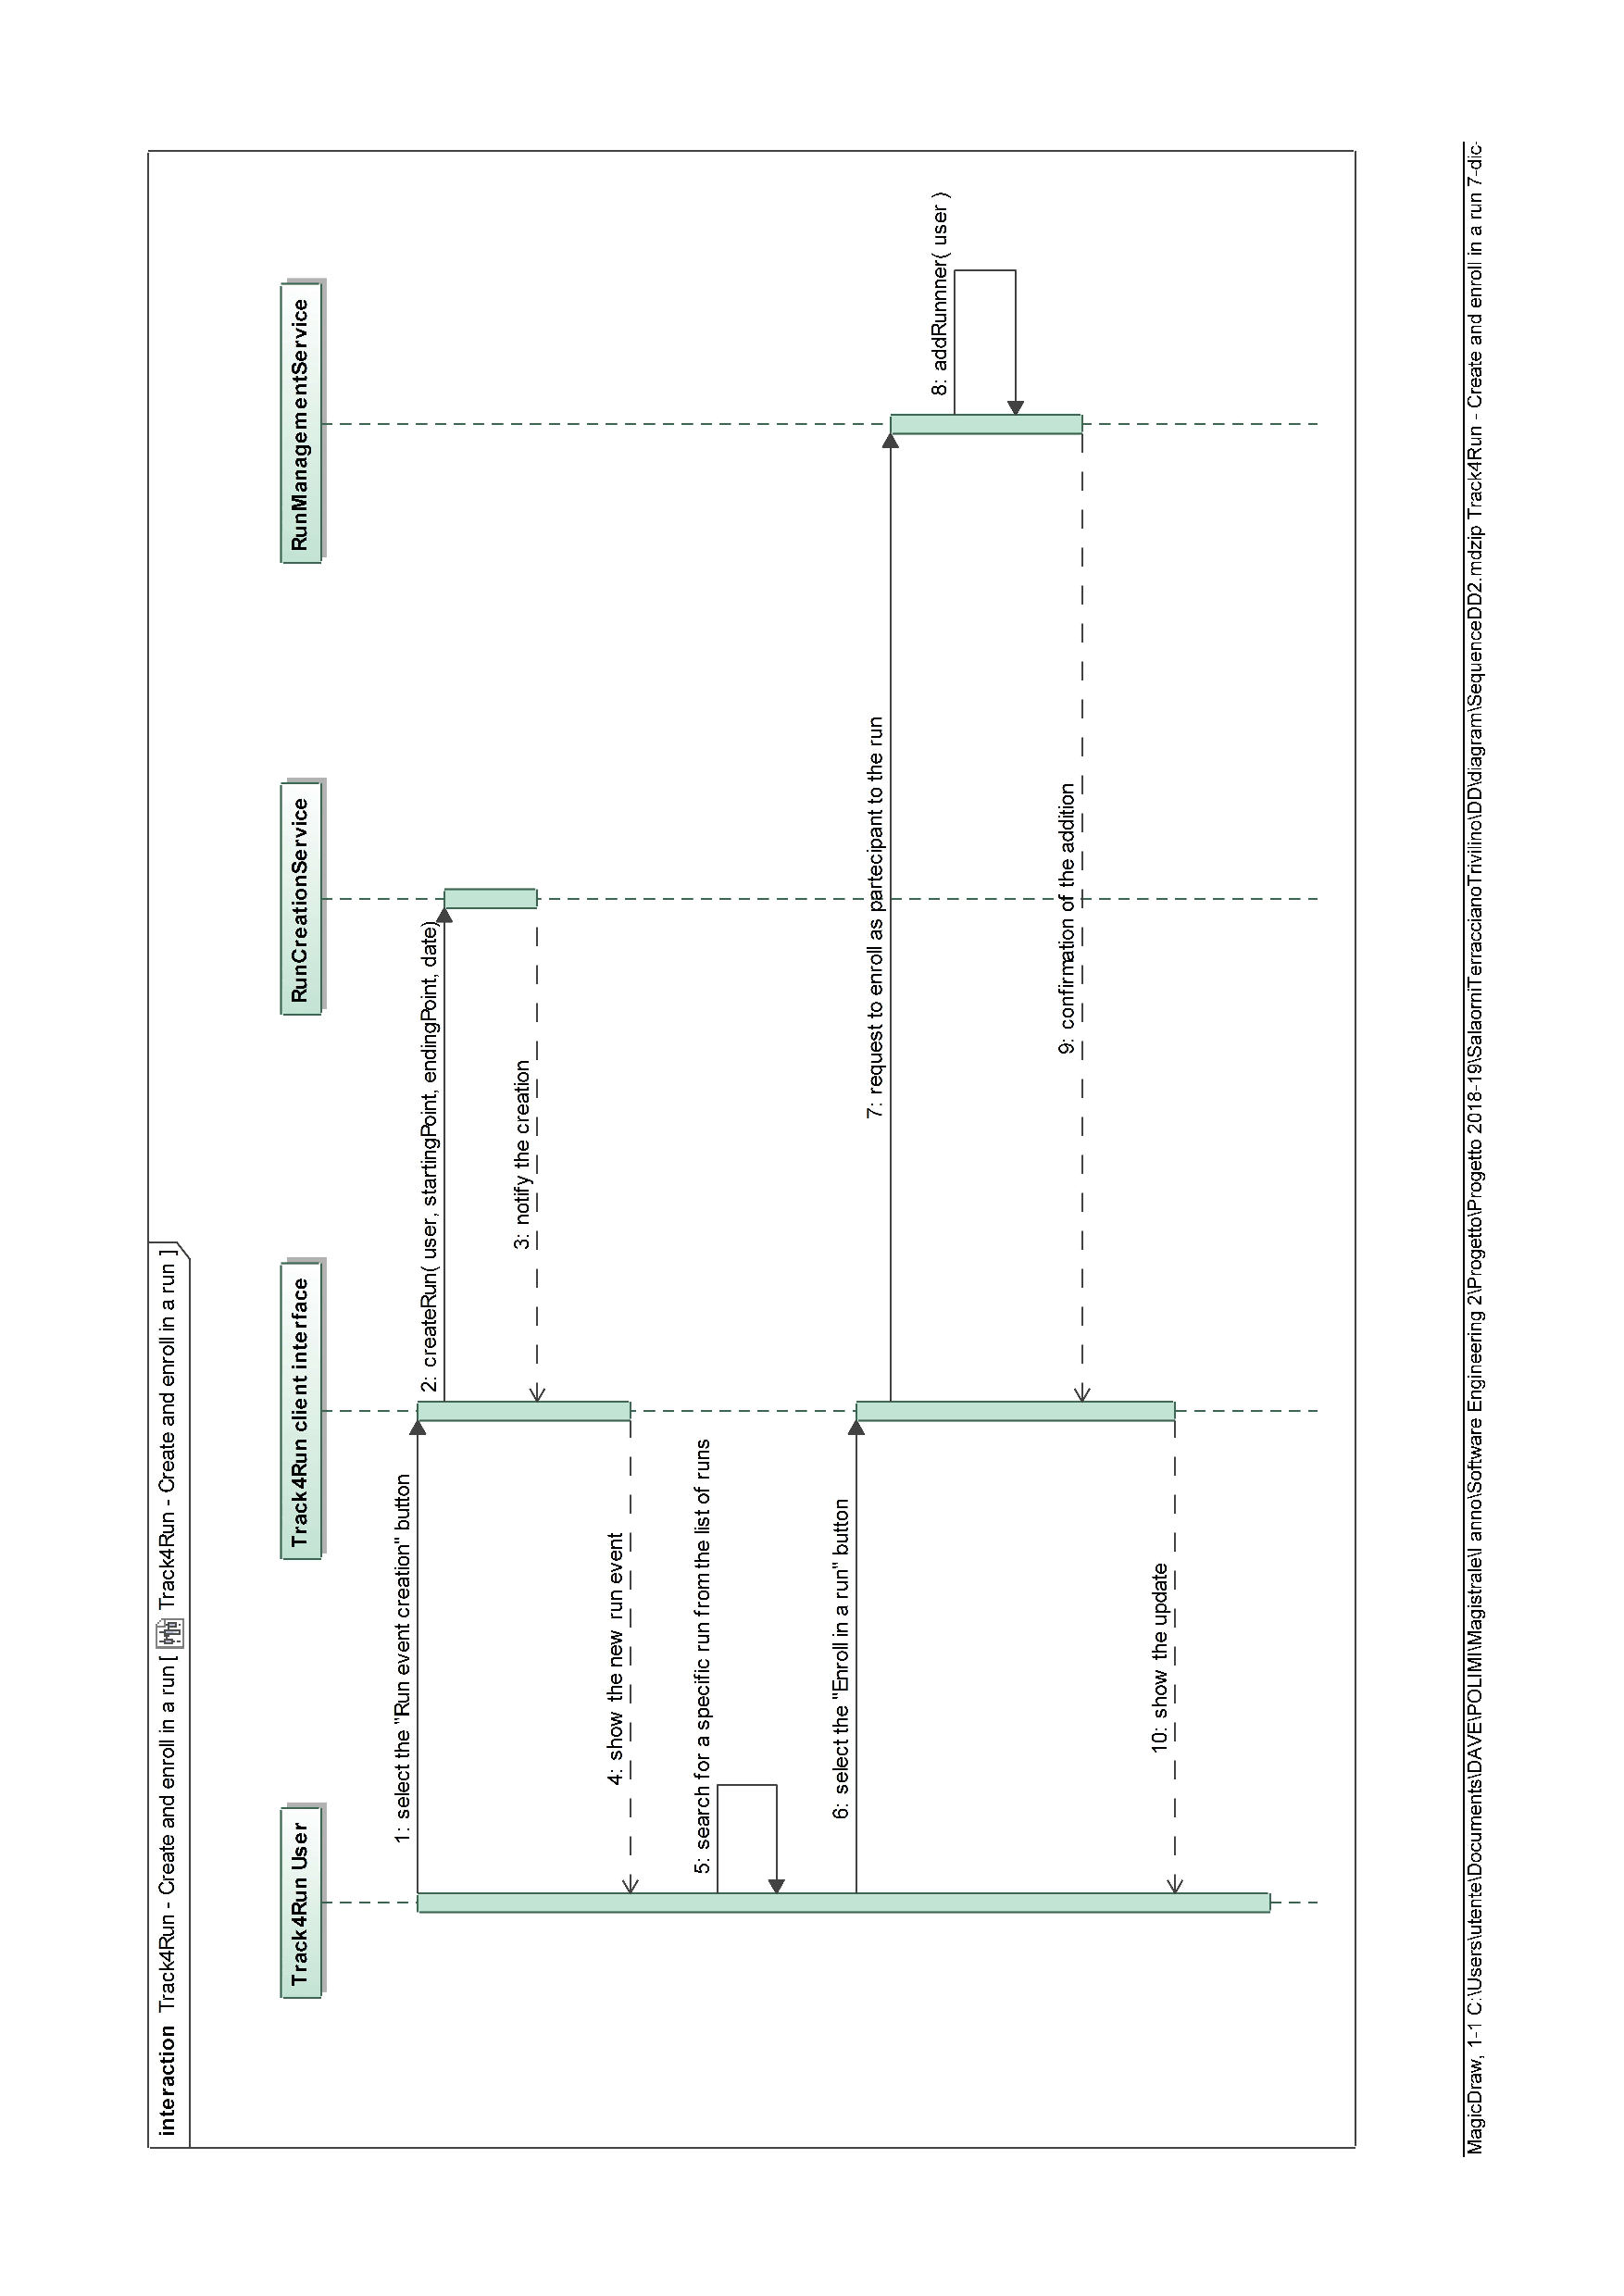
\includegraphics[width=\linewidth]{SequenceDiagram-CreateAndEnrollToARunEvent}
    \caption{Sequence Diagram showing the runtime flow.}
    \label{fig:my_label}
\end{figure}
\clearpage

\subsubsection{Track4Run - Watch a run}
When a user wants to watch a run first of all he/she sends a request to the Track4Run Server using the Client Interface, selects the run from the list obtained applying some filters (i.e. the city of the event) and then contact the Run Watch Service. \\
This component communicates with the Run Tracking Service, retrieves the position of the runners and it sends the data to the smartphone. \\
It is also possible to see the ranking of the run in real time contacting directly the Run Tracking service.

\begin{figure}[H]
    \centering
    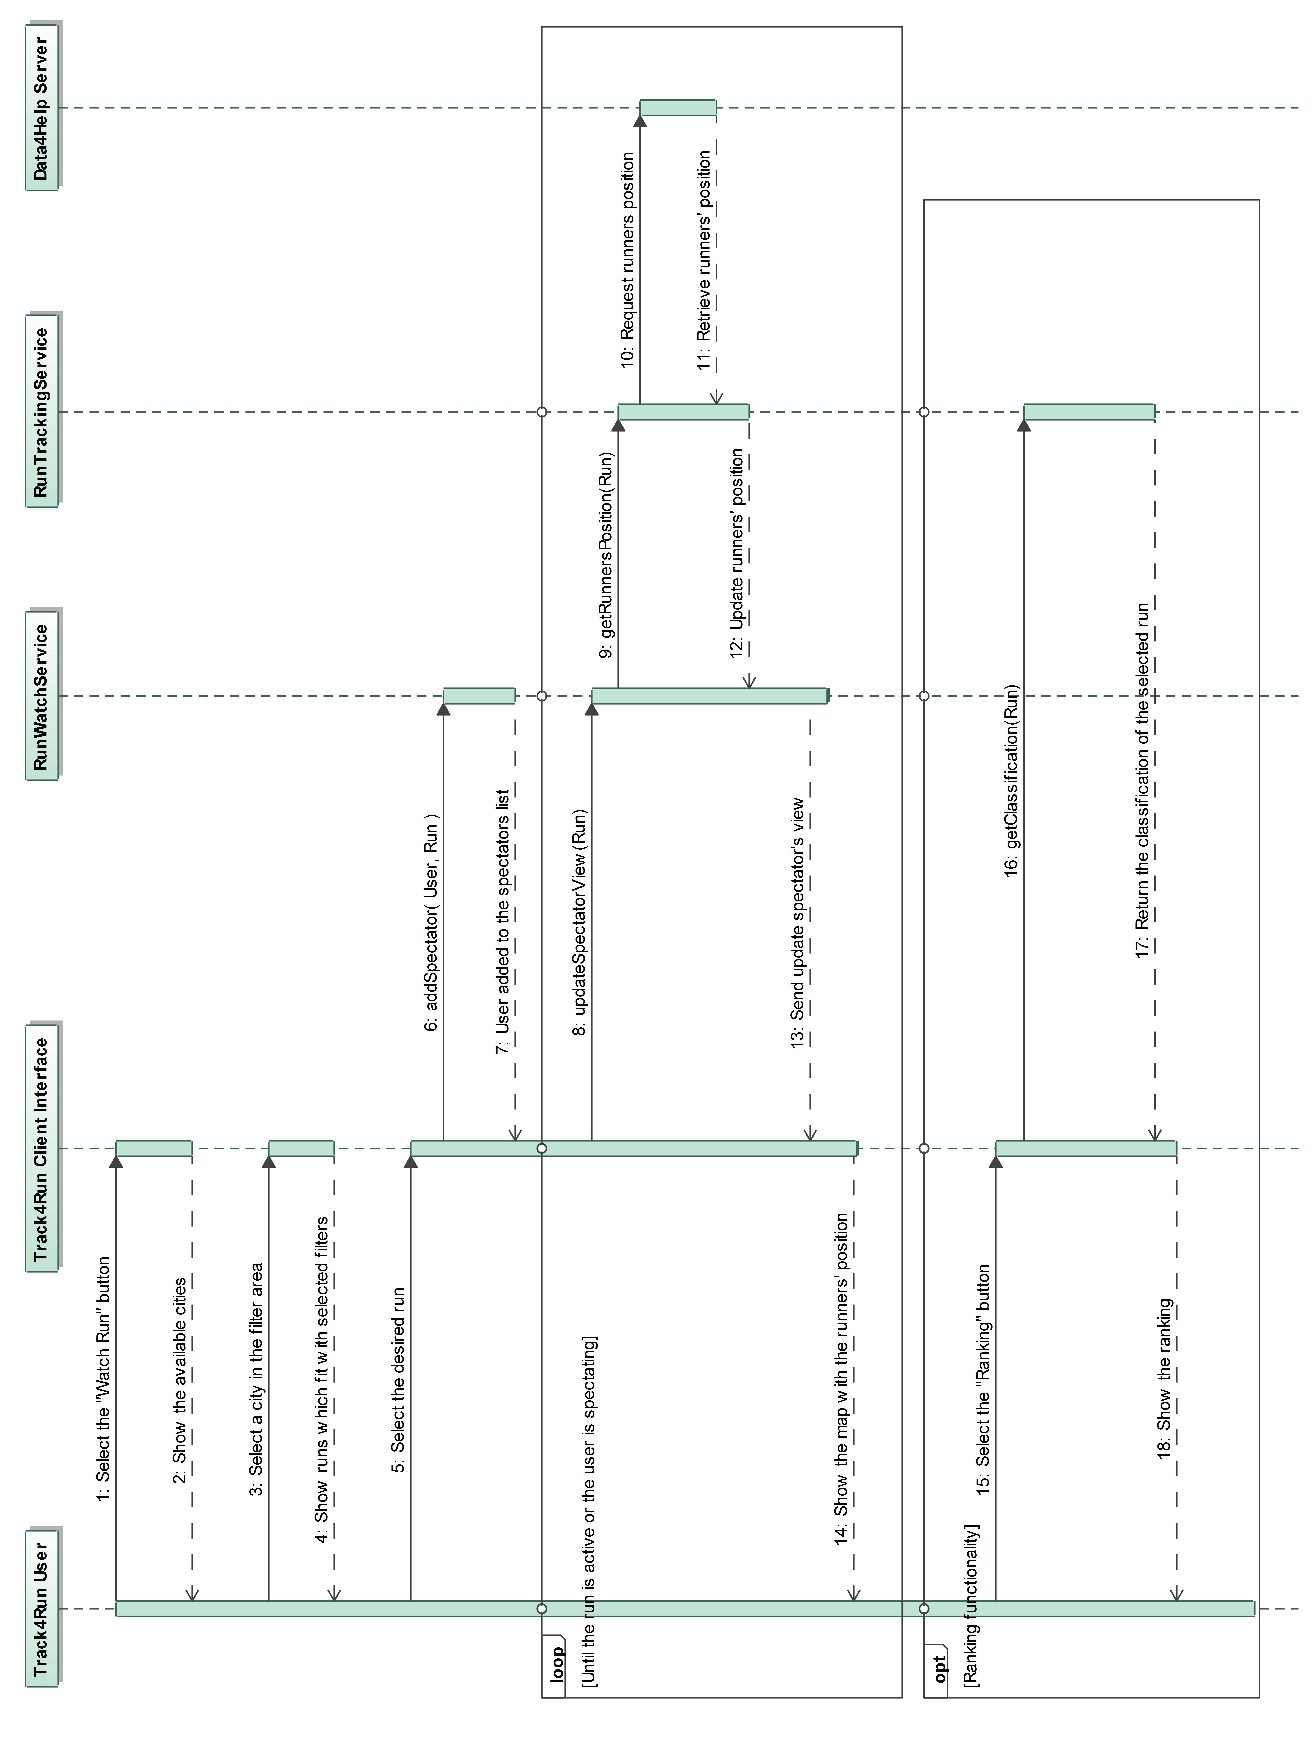
\includegraphics[width=\linewidth]{SequenceDiagram-SpectateARunEvent}
    \caption{Sequence Diagram showing the runtime flow.}
    \label{fig:my_label}
\end{figure}
\clearpage

\subsection{Component Interfaces}
This section includes further details on the interfaces between different components of the system. Their structure has been thought to hide the large amount of operations which some calls require and to maintain a good level of cohesion due to the accurate split of functionalities.\\
Here the complete diagram which shows all the interactions between the interfaces and the correct flow of each service.

\begin{figure}[H]
    \centering
    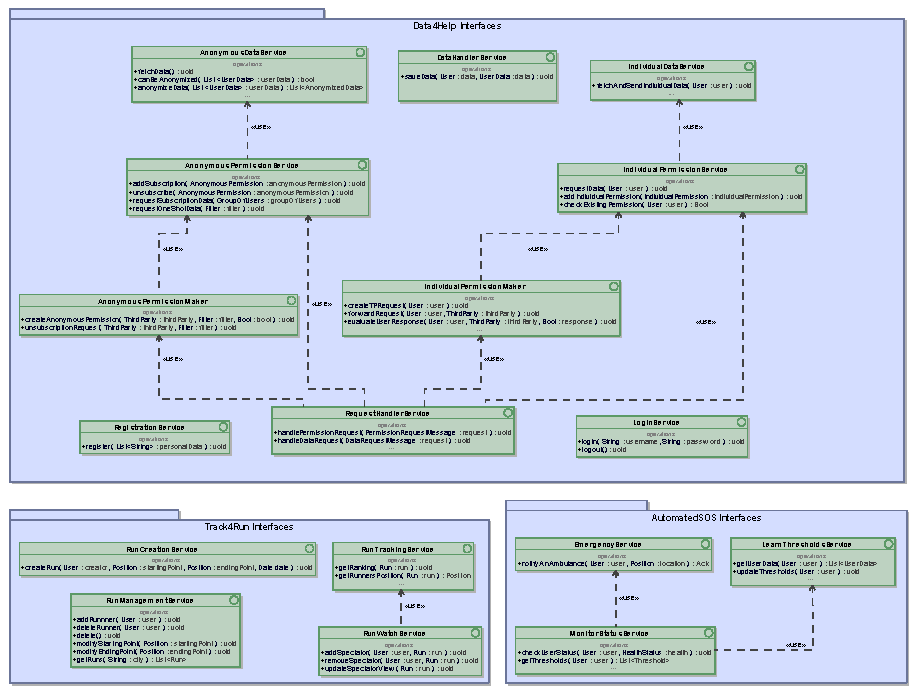
\includegraphics[width=\linewidth]{ComponentInterfaces}
    \caption{Schema with the interfaces which cover the main services.}
    \label{fig:my_label}
\end{figure}
\clearpage

\subsection{Selected Architectural Styles and Patterns}

\subsubsection{Architectural styles}
The architecture of the three applications offered by TrackMe is very similar.\\
Concerning Data4Help and Track4Run the number of tier used is three: the client, the server and the database which takes care about the presentation, the application and the data layers. \\
Since AutomatedSOS retrieves the necessary data from Data4Help and it does not have other complex data (i.e. the Run events in Track4Run) it is reasonable to delete the database for this software. \\
Regarding the data layer, it is better to keep the data storage inside the company instead of giving this layer in outsourcing, in order to safeguard the user's information due to their confidentiality. However this layer can be easily extended because of the use of interface with the database thus, if the usage of the application grows, it would be easily scalable. \\
Concerning the client solution, while Data4Help and Track4Run adopt a thin configuration, AutomatedSOS uses a thick one because it encapsulates a part of the application logic: the comparison of the health status with the threshold values.\\
This choice is guided by the fact that the software must be reactive (due to the time constraint) so, while in the server the new threshold values are periodically calculated for each user (the threshold depends on the specific user health status), the comparison must be done as soon as possible, therefore on the client side. \\ \\
The following schemata represent the different architectural styles adopted respectively for Data4Help, AutomatedSOS and Track4Run and illustrate the layer division:

\begin{figure}[H]
    \centering
    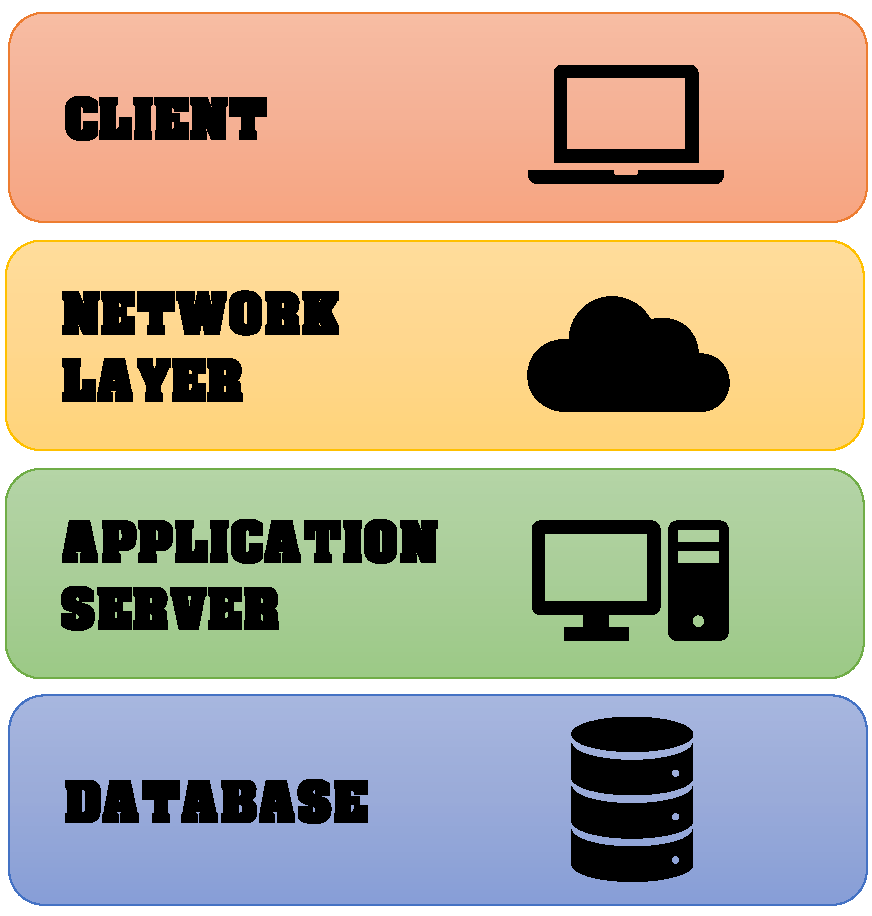
\includegraphics[width=\linewidth]{Data4Help-tier-division}
    \caption{Tier division of Data4Help system.}
    \label{fig:my_label}
\end{figure}

\begin{figure}[H]
    \centering
    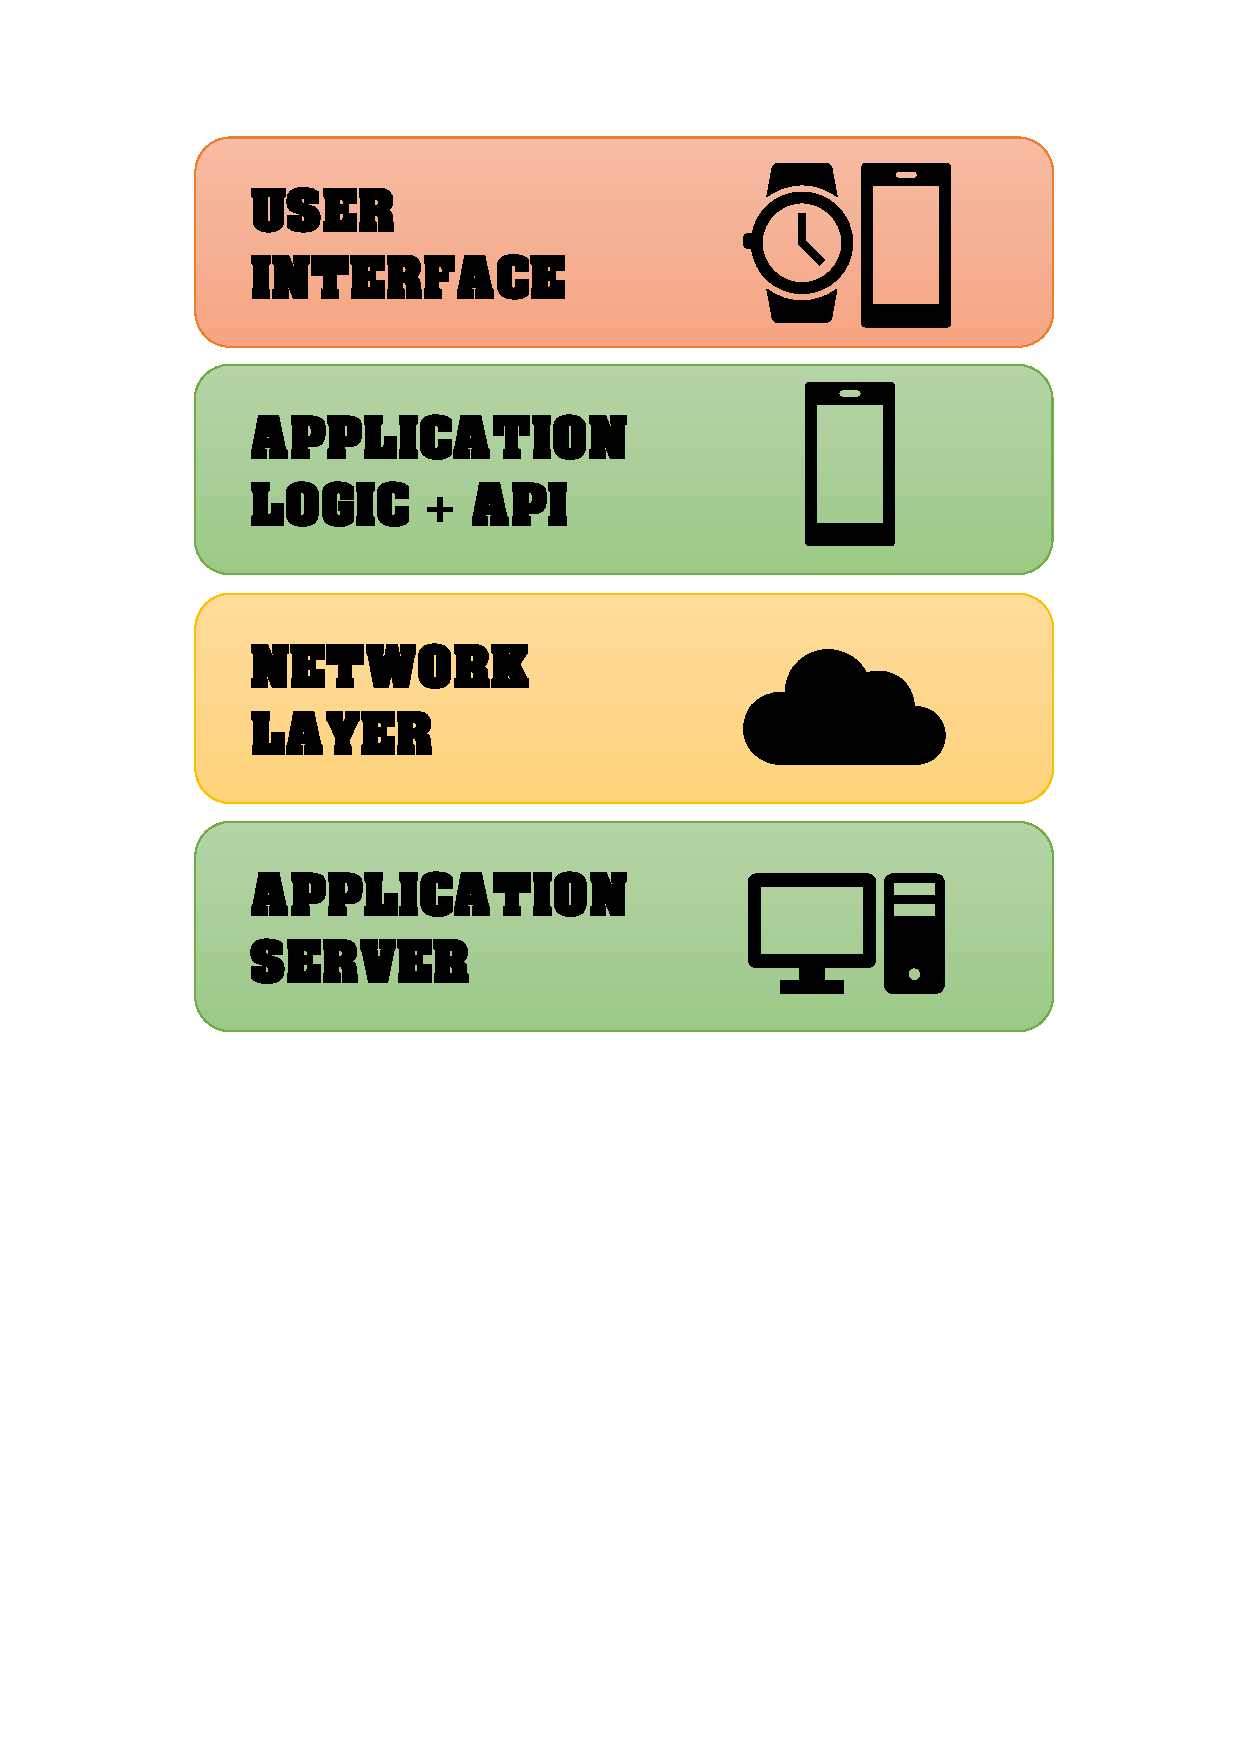
\includegraphics[width=\linewidth]{AutomatedSOS-tier-division}
    \caption{Tier division of AutomatedSOS system.}
    \label{fig:my_label}
\end{figure}

\begin{figure}[H]
    \centering
    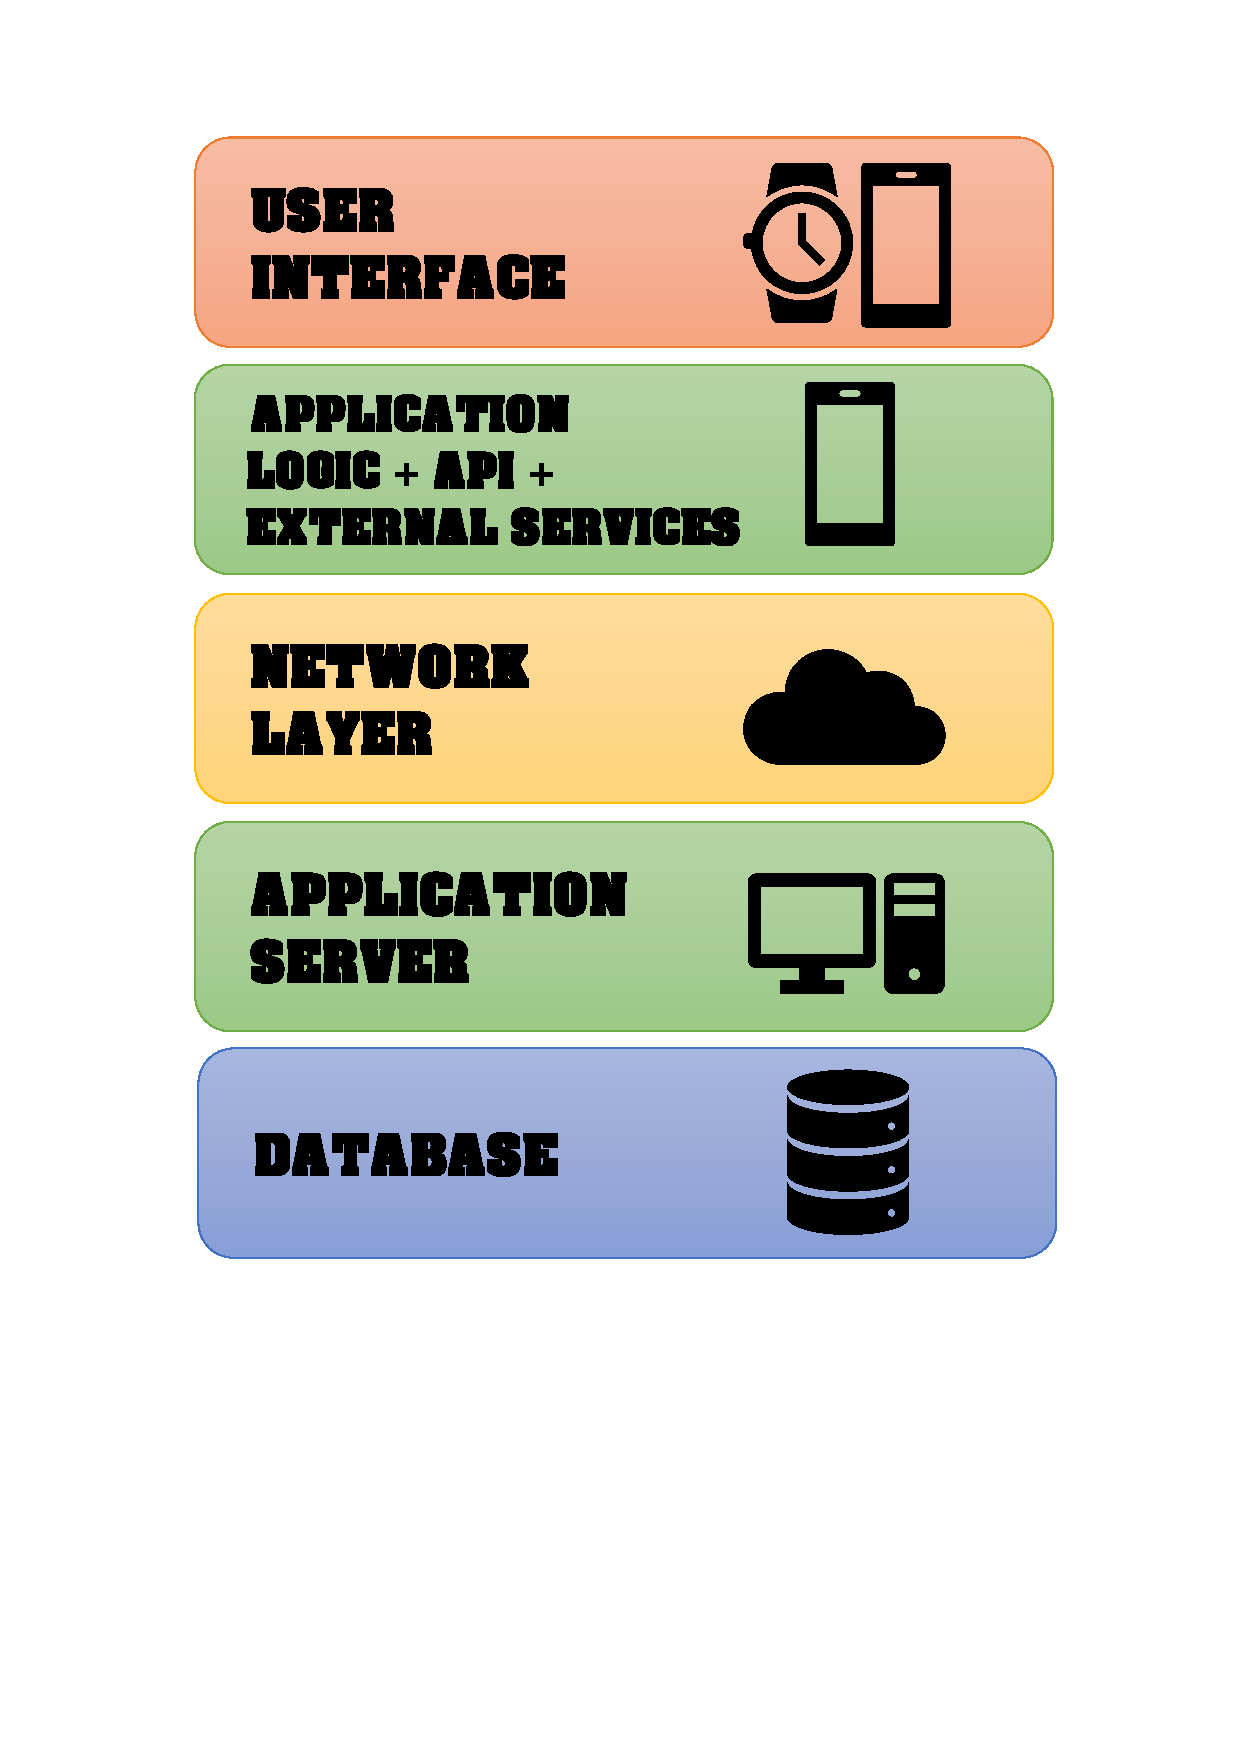
\includegraphics[width=\linewidth]{Track4Run-tier-division}
    \caption{Tier division of Track4Run system.}
    \label{fig:my_label}
\end{figure}
\clearpage

\subsubsection{Design Pattern}

\begin{itemize}
    \item \textbf{Layer Pattern:}
     Data4Help, AutomatedSOS and Track4Run are structured in layers, which simplify the split of the entire system in different groups of subtasks: presentation layer, application layer, data (persistence) layer.
     
    \item \textbf{Client-Server Pattern:} The three services are based on the Server-Client pattern. Data4Help and also AutomatedSOS and Track4Run, are composed by a server that computes the main functions, otherwise the client has the function to let the user interface to the services.
    
    \item \textbf{Model-View-Controller Pattern:} To guarantee better modularity all the services are based on the MVC pattern, the application is divided in three parts: Model, View, Controller. \\ 
    The Model lies in the servers and performs the application and persistence tasks, it is managed by the controller that lies both in server and in the clients. \\
    Finally the View, that performs the interface through which the users access and control the services, lies on the clients. This pattern allows to reduce coupling among the core functions of the services and the interface.
    
    \item \textbf{Facade Pattern:} In order to make complex subsystems easier to use and to reducing the dependencies among them, facade pattern is used in all of the three service offered by TrackMe. \\
    The main systems are divided into smaller components, they communicate with each others through interfaces. Thanks to this solution the single components do not have to touch the internal state neither to know the internal implementation of other parts.
\end{itemize}
\clearpage

\subsection{Other Design Decision}
There are some design decisions that are not treated in detail in the document. \\
First of all, concerning the communication between the server and the clients, there are several ways to do it. \\
Initially, while the application dimension is quite small, the communication part can be handled using the sockets and then, once the application grows, a middleware can be used to hide some complexity factors (i.e. see Java RMI).\\
In fact, while the application grows, is necessary to introduce more endpoints and distribute them in order to balance all the requests that has to be handled.\\
Another question that needs a note is derived by the choice of the communication type to adopt.\\
An intuitive option is to use a message-based communication model.
This decision is primarly supported by the adoption of the Visitor design pattern. \\
In fact, the use of specific classes of messages offers to the developers the possibility to divide the various messages handling methods and it also relieves the dimension of all the classes which unpack the messages. 
This can be done encapsulating some methods in the message itself.
\\ 
Regarding the database technology adopted, there is a huge variety of solutions.\\
One peculiar option is to use, instead of a traditional database solution, a middleware that manages data in an efficient way.\\
One of these could be Apache Flink which is a distributed stream and batch data processing system. This middleware also provides a set of API to enable SQL query and actually transform the distributed application in an efficient query system to retrieve a large amount of data.
\clearpage

\section{User Interface Design}
The user interface design has been already illustrated in the RASD in section 3.1.1 where have been presented the main mock-ups of the applications.\\
Since weren't done relevant modifications on the typology and the presentation of the interfaces, each link with the application view refers to those mock-ups. 
\vspace{.5cm}

\section{Requirements Traceability}

\begin{enumerate}[label*=\bf{R.\arabic*}]

\item - People can create a user account selecting username, password,
giving personal information (age, address,gender) and allow to
share their anonymized data.

\begin{itemize}
\item RegistrationService
\end{itemize}

\item - It is possible to create a third party account selecting username
and password and giving the company main information.

\begin{itemize}
\item LoginService
\end{itemize}

\item - Data4Help allows third parties to request anonymized data acquired
from a filtered group of users (by age, gender, address, etc.).

\begin{itemize}
\item RequestHandlerService
\end{itemize}

\item Data4Help collects data from registered users and gives access to
third parties only if the number of individuals whose data satisfy the
request is higher than 1000.

\begin{itemize}
\item RequestHandlerService
\item AnonymousPermissionMaker
\item AnonymousPermissionService
\item AnonymousDataService
\end{itemize}

\item - Data4Help allows third parties to join the subscription service for an
indeterminate period and then, in case, unsubscribe from that.

\begin{itemize}
\item RequestHandlerService
\item AnonymousPermissionMaker
\item AnonymousPermissionService
\end{itemize}

\item - Data4Help provides new data, checking each time if groups data satisfy the given constraint (number of individuals not lower than a
thousand).

\begin{itemize}
\item AnonymousDataService
\end{itemize}

\item - Data4Help keeps track of the associations between third parties subscriptions and the required group data.

\begin{itemize}
\item AnonymousPermissionService
\end{itemize}

\item - Data4Help allows third parties to require specific person’s data.

\begin{itemize}
\item RequestHandlerService
\end{itemize}

\item - Data4Help forwards requests from third parties to the demanded users which can accept or refuse to share their own personal data.

\begin{itemize}
\item IndividualPermissionMaker
\end{itemize}

\item - Data4Help keeps track of the connections between a specific user and the third parties which can access to his/her data.

\begin{itemize}
\item RequestHandlerService
\item IndividualPermissionService
\item IndividualDataService
\end{itemize}

\item - Data4Help allows third parties to have access to demanded users’ data each time they need them.

\begin{itemize}
\item RequestHandlerService
\item IndividualPermissionService
\item IndividualDataService
\end{itemize}

\item - Users’ health and position information received from Data4Help data collector process are analyzed and compared with the threshold values.

\begin{itemize}
\item MonitorStatusService
\item LearnThresholdsService
\end{itemize}

\item - In case of emergency (the health status values overcome the threshold) a request for an ambulance is sent to the ambulance dispatcher in 5 seconds, containing the user’s information.

\begin{itemize}
\item EmergencyService
\end{itemize}

\item - Users select the day, the hour at which the run begins, the starting point, the ending point and the path for the run.

\begin{itemize}
\item RunCreationService
\end{itemize}

\item - The run event is stored in the system in order to be managed during its lifecycle.

\begin{itemize}
\item RunManagementService
\end{itemize}

\item - Users can browse among the available runs and see their information.

\begin{itemize}
\item RunManagementService
\end{itemize}

\item - Users can choose a run and register to it as a runners.

\begin{itemize}
\item RunManagementService
\end{itemize}

\item - The system saves the enrolled users as runners and keeps track of the association with the run event.

\begin{itemize}
\item RunManagementService
\end{itemize}

\item - The system keeps track of all the enrolled runners’ position during the run.

\begin{itemize}
\item RunTrackingService
\end{itemize}

\item - Users who require to watch a run are saved as spectators to the run event.

\begin{itemize}
\item RunWatchService
\end{itemize}

\item - Track4Run offers the possibility to see the run live through a map.

\begin{itemize}
\item RunWatchService
\item RunTrackingService
\end{itemize}

\end{enumerate}
\clearpage

\section{Implementation, Integration and Test Plan}
\subsection{Implementation Plan}
The core service developed by TrackMe is Data4Help. In fact the Third parties services, and also AutomatedSOS and Track4Run, are developed on top of Data4Help. 
It is a reasonable strategy plan to start the implementation from Data4Help and then to proceed with AutomatedSOS and Track4Run.

\begin{figure}[H]
    \centering
    \includegraphics[width=\linewidth]{BuildPlanStack}
    \caption{TrackMe software stack organization.}
    \label{fig:my_label}
\end{figure}

\begin{enumerate}[label*=\bf{\arabic*.}]

\item \textbf{Data4Help} First of all, the model of our application has to be developed in order to provide a basement to all the services that will run in Data4Help. Since the main functions of the application are all based on data management, it is useful that the building process starts from the two services that involves the data and their relation with the database: Individual and Anonymous Data Service and DMBS integration [1.1].\\
Once the data management is implemented, the next proposed section that has to be developed is the one devoted to manage the permission and access to the data: the Individual and the Anonymous Permission Service [1.2].
The next step is to implement the services which create the permissions: the Individual and the Anonymous Permission Maker [1.3]. Finally, the development of the model implementation can be concluded with the login, the registration and the service that manages requests received from the third parties. These services are called: RequestHandlerService [1.4], LoginService and RegistartionService [1.5].\\
When the model is completed, the implementation can continue with the Data Collector, the service that is integrated with third party mobile apps, devoted to collect the users' data and send them to data4Help server [1.6].\\ 
Finally the web interface [1.7] can be developed.


\begin{enumerate}[label*=\bf{\arabic*}]
    \item \textbf{Model} - IndividualDataService, AnonymousDataService, DBMS, Database
    \item \textbf{Model} - IndividualPermissionService, AnonymousPermissionService, 
    \item \textbf{Model} - IndividualPermissionMaker, AnonymousPermissionMaker
    \item \textbf{Model} - RequestHandlerService
    \item \textbf{Model} - LoginService, RegistrationService
    \item \textbf{Model-Controller} - Data Collector for the third party applications
    \item \textbf{View} - Web interface
\end{enumerate}

\item \textbf{AutomatedSOS}
As regards AutomatedSOS, the implementation should start from the model, in particular from the server services involved in data receipt and the users' thresholds evaluation [2.1]: LearnThresholdsService.\\
Then  can be implemented the service which manages the emergency status and the ambulance call [2.2]: the EmergencyStatusService.\\
Finally, the Client side which has to be developed is composed by: the mobile App [2.3], the integration with the Data4Help Collector and the the MonitorStatusService, [2.4] that checks the user's status.

\begin{enumerate}[label*=\bf{.\arabic*}]
    \item \textbf{Model-Controller} - LearnThresholdsService and communication with Data4Help
    \item \textbf{Model-Controller} - EmergencyStatusService and communication with Ambulance Dispatcher
    \item \textbf{Model-View-Controller} Mobile Application and communication
    \item \textbf{Model} MonitorStatusService
\end{enumerate}

\item \textbf{Track4Run}
Also for Track4Run the implementation should start from the model. At first is developed the database [3.1], followed by the main service which manages the run events [3.2] and the service to create them [3.3]: the RunManagementService and the RunCreationService.\\
Then, the service involved in data receipt, position tracking and communication with external service can be implemented [3.4]: this is the RunTrackingService. To conclude the model implementation, can be developed the service to manage the run watching [3.5]: RunWatchService.\\
Finally can be developed the mobile app with the integration with the Data4Help Colector [3.6].

\begin{enumerate}[label*=\bf{.\arabic*}]
    \item \textbf{Model} database
    \item \textbf{Model} RunManagementService
    \item \textbf{Model}RunCreationService
    \item \textbf{Model- Controller} RunTrackingService and communication with External Actors
    \item \textbf{Model} RunWatchService
    \item \textbf{View-Controller} Mobile App and communication
\end{enumerate}
\end{enumerate}

\subsection{Integration and Testing}

\subsubsection{Testing Strategy}
It is highly recommended to start the testing phase as soon as the development begins in order to reduce the possibility to increase the risk of high cost of repairing during the implementation. For this reason, a strategy based on a Big Bang approach can be risky, instead an incremental one could be more appropriate.\\ \\
Since the implementation plan has to start from the basic services proceeding incrementally to the top services, it is a reasonable decision to carry out a \textit{bottom-up strategy} for the integration testing.\\
Thanks to this solution the testing phase can start since the first moment of the implementation. As soon as the components are implemented, they can be tested through the use of drivers. Then, when also upper components are developed, the integration among them can be tested, and so on.\\ \\
Furthermore, since all the functionalities are implemented by specific and modular services and the communication among them is granted by the use of interfaces, a low level of coupling is guaranteed and this allows to facilitate the integration testing.

\subsubsection{Integration Testing Plan}

\paragraph{Data4Help}
The integration testing for Data4Help ha to be executed between the following components:

\begin{itemize}
    \item Application Server with the DBMS
    \item Application Server with Third Parties
    \item Application Server with Data Collector API
    \item Application Server with Web interface
    \item Between the internal Application Server components
\end{itemize}

\noindent As mentioned before, the integration testing is based on the bottom-up approach. For this reason the testing starts from the integration test of the application components with the database, that is the first component developed in the implementation plan.\\
In fact, the testing phase can start as soon as the component of a specific level, or also a single function, is completed and proceeds incrementally in order to test the integration with upper components, also using specific drivers.\\
After the integration with the database, the testing can proceed with the model services, that manage the permissions, both anonymous and individual, and then with the service that handle the data and permission request.\\ 
Finally, are tested the integration between the client and the server : the server with the Data Collector to take data from the devices and the server with the web page.
\newline \newline This is the order in which the integration test for Data4Help should be carried on:


\begin{enumerate}[label*=\bf{\arabic*} . ]
    \item Database - AnonymousDataService
    \item Database - IndividualDataService
    \item Database - DataHandlerService
    \item AnonymousDataService - AnonymousPermissionService
    \item IndividualDataService - IndividualPermissionService
    \item IndividualPermissionService - IndividualPermissionMaker
    \item AnonymousPermissionService - AnonymousPermissionMaker
    \item IndividualPermissionService - RequestHandlerService
    \item AnonymousPermissionService - RequestHandlerService
    \item AnonymousPermissionMaker - RequestHandlerService
    \item IndividualPermissionMaker - RequestHandlerService
    \item DataCollectorService - DataHandlerService
    \item Web interface - LoginService
    \item Web interface - RegistrationService
\end{enumerate}

\paragraph{AutomatedSOS}
The integration testing for AutomatedSOS have to be executed between the following components:
\begin{itemize}
    \item Application Server with the Mobile App
    \item Application Server with Data4Help
    \item Application Server with Ambulance Dispatcher
    \item Mobile App with Data4Help Data Collector
\end{itemize}

\noindent Also for AutomatedSOS the integration testing starts from the main server services. At first is tested the integration between the server and Data4Help, then the one between the server and the ambulance dispatcher service.\\
Finally the integration between the client and the server, especially between the MonitorStatusService (client) and the EmergencyStatusService (server) and between the MoitorStatusService and the Data4Help Data Collector (Data4Help API).
\newline\newline This is the order in which the integration test for AutomatedSOS should be done:

\begin{enumerate}[label*=\bf{\arabic*} . ]
    \item LearnThresholdsService - Data4Help
    \item EmergencyStatusService - Ambulance Dispatcher external service
    \item EmergencyStatusService - MonitorStatusService
    \item MonitorStatusService - Data4Help Data Collector
\end{enumerate}

\paragraph{Track4Run}
The integration testing for Track4Run have to be executed between the following components:

\begin{itemize}
    \item Application Server with the Mobile App
    \item Application Server with Data4Help
    \item Application Server with DBMS
    \item Application Server with external services (i.e. Google Maps)
    \item Mobile App with Data4Help Data Collector
    \item Between the internal Application Server components
\end{itemize}

\noindent Following the implementation plan, the first component to be tested is the database and its integration with the several application server services, then the integration between the server and Data4Help and the external services.\\
Finally, once the client app is implemented, the testing can proceed with the integration between Mobile app and Data4Help Data Collector and Mobile app and application server.
\newline\newline This is the order in which the integration test for Track4Run should be done:

\begin{enumerate}[label*=\bf{\arabic*} . ]
    \item RunManagementService - Database
    \item RunCreationService - Database
    \item RunTrackingService - Database
    \item RunWatchService - Database
    \item RunTrackingService - Data4Help
    \item RunTrackingService - External Services (Google maps)
    \item Mobile App - Data4Help Data Collector
    \item RunManagementService - Mobile App
    \item RunCreationService - Mobile App
    \item RunTrackingService - Mobile App
    \item RunWatchService - Mobile App
\end{enumerate}

\clearpage

\section{Effort Spent}

Davide Salaorni

\begin{center}
\begin{tabular}{|l | l |}
    \hline \bf{Purpose, Scope, Definitions} & 2 \\ \hline
    \bf{High level Architecture}  & 3 \\ \hline
    \bf{Component Interface} & 6 \\ \hline
    \bf{Deployment View} & 3 \\ \hline
    \bf{Run Time View} & 5\\ \hline
    \bf{Component View} & 4 \\ \hline
    \bf{Architectural Style and Pattern} & 2 \\ \hline
    \bf{Requirement Traceability} & 2 \\ \hline
    \bf{Implementation, Integration and Testing} & 2 \\ \hline
\end{tabular}
\end{center}

Luca Terracciano

\begin{center}
\begin{tabular}{|l | l |}
    \hline \bf{Purpose, Scope, Definitions} & 1 \\ \hline
    \bf{High level Architecture}  & 2 \\ \hline
    \bf{Component Interface} & 6 \\ \hline
    \bf{Deployment View} & 7 \\ \hline
    \bf{Run Time View} & 2\\ \hline
    \bf{Component View} & 4 \\ \hline
    \bf{Architectural Style and Pattern} & 4 \\ \hline
    \bf{Requirement Traceability} & 2 \\ \hline
    \bf{Implementation, Integration and Testing} & 2 \\ \hline
\end{tabular}
\end{center}

Manuel Trivilino

\begin{center}
\begin{tabular}{|l | l |}
    \hline \bf{Purpose, Scope, Definitions} & 1 \\ \hline
    \bf{High level Architecture}  & 4 \\ \hline
    \bf{Component Interface} & 6 \\ \hline
    \bf{Deployment View} & 1 \\ \hline
    \bf{Run Time View} & 4\\ \hline
    \bf{Component View} & 3 \\ \hline
    \bf{Architectural Style and Pattern} & 4 \\ \hline
    \bf{Requirement Traceability} & 2 \\ \hline
    \bf{Implementation, Integration and Testing} & 5 \\ \hline
\end{tabular}
\end{center}
\clearpage

\section{References}
\begin{itemize}
    \item Mandatory Project Assignment AY 2018-2019
    \item Slides from the lectures
    \item IEE Standard for Information Technology - Software Design Description
    \item IEE Standard for Systems and Software Engineering - Architecure Description
    \item Deployment diagrams documentation - https://www.uml-diagrams.org/deployment-diagrams.html
\end{itemize}

\end{document}
